\documentclass {report}

\usepackage[utf8]{inputenc}
\usepackage[T1]{fontenc}
\usepackage[francais]{babel}
\usepackage{url}
\usepackage{lmodern}
\usepackage{fancyhdr}
\usepackage{listings}
\usepackage{color}
\usepackage{graphicx}
\usepackage{caption}
\usepackage{xcolor}
\usepackage[top=2.5cm, bottom=2cm, left=3cm, right=2cm]{geometry}
\usepackage{lettrine}
\usepackage{multicol}
\usepackage{amssymb}
\DeclareGraphicsExtensions{.png,.pdf,.eps}
\usepackage{pstricks}

\definecolor{mygreen}{rgb}{0,0.6,0}
\definecolor{mygray}{rgb}{0.5,0.5,0.5}
\definecolor{mymauve}{rgb}{0.58,0,0.82}


\def\thickhrulefill{\leavevmode \leaders \hrule height 0.5pt\hfill \kern}
\def\blurb{%
  Université de Technologie de Compiègne \\
  Septembre 2013 - février 2014} 
\def\clap#1{\hbox to 0pt{\hss #1\hss}}%
\def\title#1{%
  \hbox to \hsize{%
    \vbox{\centering #1}}}%
\def\ligne#1{%
  \hbox to \hsize{%
    \vbox{\raggedright #1}}}%
\def\haut#1#2#3{%
  \hbox to \hsize{%
    \rlap{\vtop{\raggedright #1}}%
    \hss
    \clap{\vtop{\centering #2}}%
    \hss
    \llap{\vtop{\raggedleft #3}}}}%
\def\bas#1#2#3{%
  \hbox to \hsize{%
    \rlap{\vbox{\raggedright #1}}%
    \hss
    \clap{\vbox{\centering #2}}%
    \hss
    \llap{\vbox{\raggedleft #3}}}}%


\begin{document}
%%configuration de listings
\lstset{
language = python,
basicstyle=\footnotesize,
tabsize=4,
frame = tBlR ,
rulesep =1 mm ,
framesep =5 mm ,
framerule =2 pt ,
xrightmargin =5 mm ,
xleftmargin =5 mm ,
rulecolor ={\color[gray]{0.6}},
rulesepcolor ={\color[gray]{0.9}},
showstringspaces=false,
commentstyle=\color{mygreen},
keywordstyle=\color{blue},
numberstyle=\tiny\color{mygray},
stringstyle=\color{mymauve}
}

\begin{titlepage}
\thispagestyle{empty}\vbox to .9\vsize{%
  
\includegraphics[scale=0.7]{logilab.png} 
  \hfill
  
\includegraphics{utc.png} 
  \vss
  \vbox to 1\vsize{%
    \haut{}{\blurb}{}
    
    \vfill
    \title{
    \Large Mise en place de moteurs d'inférences dans la plateforme CubicWeb}
    \vspace{5mm}
    \hrule height 0.5pt
    \vspace{5mm}
    \title{\Large Léa \textsc{Capgen} GI03 ICSI}
    \vskip 1cm
    \vfill
    \ligne{%
      \begin{tabular}{l}
        Sous la direction de : \\
      \end{tabular}}
    \vspace{2mm}
    \ligne{%
      \begin{tabular}{l}
        M. Vincent \textsc{Michel} Logilab (tuteur) \\
        M. Gérard \textsc{Govaert} UTC (enseignant suiveur)\\
      \end{tabular}
        }
    \vskip 1cm
    \vfill
    
    \bas{}{Logilab, 104 boulevard Auguste Blanqui, Paris 13ème \\
           \url{http://logilab.fr}}{}
    }%
  \vss
}
\end{titlepage}

\chapter*{Remerciements}

\paragraph{}
Je tiens à remercier Monsieur Vincent Michel, chef de projet au sein du département Web sémantique et tuteur de ce stage, pour la confiance et l'autonomie qu’il m’a accordées dès mon arrivée dans l’entreprise, pour les conseils qu'il m'a apportés lors des différents suivis, et pour le temps qu'il m'a consacré. Je remercie également Monsieur Gérard Govaert, enseignant suiveur de l'UTC, pour sa visite sur le lieu du stage. 
\paragraph{}
Je tiens à témoigner ma reconnaissance aux personnes suivantes: Monsieur Olivier Cayrol, directeur adjoint de Logilab, pour son intégration au sein de l'entreprise et ses conseils sur la communication du projet au sein de la communauté CubicWeb; Messieurs Nicolas Chauvat, PDG de l'entreprise Logilab, Adrien Di Mascio, directeur du Département Web sémantique, Sylvain Thénault, Directeur de l'Agence de Toulouse et Anthony Truchet, chef de projet au sein du département Informatique Scientifique,  pour l'intérêt qu'ils ont porté au sujet de mon stage ; Madame Katia Saurfelt, chef de projet au sein du Département Web Sémantique, pour sa gentillesse, l'accueil au sein de son bureau et son aide tout long de ce stage; Monsieur Alain Leufroy, chef de projet au sein du Département Informatique scientifique, pour sa formation sur le Python scientifique et sa bonne humeur quotidienne; ainsi que l'ensemble du personnel de Logilab pour sa sympathie et son accueil.



\chapter*{Résumé technique}
\paragraph{}
Le stage que j'ai effectué s'est déroulé au sein du département “Web Sémantique” de Logilab, entreprise spécialisée dans l’informatique numérique et la gestion des connaissances. Logilab propose des outils de gestion de connaissances basés sur le logiciel libre CubicWeb. Le sujet de ce stage porte sur la mise en place d'inférences sur la plateforme CubicWeb, à la base de la création des applications produites par Logilab. Il s'agit d'offrir la possibilité de traiter l'ensemble des données d'une application avec des règles, en vue d'en extraire des nouvelles informations pertinentes. Afin de mettre en place un mécanisme de règles, mon stage s'est principalement articulé autour de deux actions : la mise en place d'un système expert et la mise en place de règles pour permettre une réécriture de requêtes RQL, langage d'interrogation et de modification de données.
\paragraph{}
Dans un premier temps, la réalisation d'un système expert avec Pyke a permis d'inférer sur les données de l'application. Pyke est un moteur d'inférences écrit en Python qui introduit de la programmation logique inspirée de Prolog. La base de faits est composée des données de la base de données de l'application. Les données inférées selon les règles mises en place peuvent alors être intégrées à la base de données ou stockées séparément. Dans le cadre de la plateforme CubicWeb, les règles suivent un algorithme de chaînage-avant par saturation. Afin de réaliser ce système expert, mes compétences en matière d'algorithmique et de programmation logique ont été sollicitées.
\paragraph{}
Dans un deuxième temps, la mise en place de règles au niveau de la modélisation des données a pour objectif de faciliter l'interrogation de la base de données et d'en extraire de nouvelles données déduites de celles existantes. Ce mécanisme, apportant de la flexibilité à la modélisation de données, a nécessité des ajouts de fonctionnalités à la plateforme CubicWeb et de mettre en œuvre un mécanisme de réécriture de requêtes RQL. En effet, le RQL utilise des règles définies dans le modèle de données afin d'accéder aux données déduites de cette règle. Pour cela, il m'a fallu comprendre et manipuler le graphe de requêtes RQL.
\paragraph{}
Les méthodologies et outils, utilisés tout au long de ses vingt-quatre semaines, sont une méthode de développement logiciel agile, le \textit{test driven development}, Mercurial, Python, Javascript, CubicWeb, Debian.

\tableofcontents


\clearpage
\begin{flushright}
\begin{minipage}[c]{7cm}
\chapter*{Introduction}
    \lettrine{L}{es stages en entreprise} ou laboratoire font partie intégrante de la formation d’ingénieur de l’Université de Technologie de Compiègne (UTC). La finalité essentielle est d'acquérir une expérience dans le milieu professionnel, afin de s'initier à la pratique du métier d’ingénieur et d'en saisir les enjeux. Les travaux confiés sont l’occasion de développer mes connaissances et de mettre en application les enseignements théoriques et pratiques reçus ainsi que de développer mes facultés d’adaptation, d’analyse et de synthèse. Ce premier stage de six mois a eu lieu au sein de l’entreprise Logilab du 2 septembre 2013 au 14 février 2014, dans le département Web sémantique. Logilab est une entreprise d'une vingtaine de personnes qui développe des logiciels, propose du conseil et des formations de haut niveau dans les domaines de l’informatique scientifique et du Web sémantique. Ce rapport vise à présenter l'entreprise, la méthodologie employée, les travaux effectués, ainsi que mon retour d'expérience.
\end{minipage}
\end{flushright}
\pagestyle{headings}


\part{Présentation de l'entreprise}

\chapter{Logilab : une entreprise acteur du logiciel libre}
\section{Activité et domaines de compétences}
\paragraph{}
Logilab est une société anonyme d'une vingtaine de personnes créée en septembre 2000 dont l'activité consiste à développer des logiciels, les intégrer dans les systèmes d'information clients et à proposer du conseil et des formations de haut niveau dans les domaines de l'informatique scientifique et du Web sémantique\footnotemark[1]. Les principales formations proposées par Logilab concernent la programmation Python, la programmation scientifique en Python (e.g analyse de données, statistiques, fouilles de données, calcul numérique), programmation d'interfaces graphiques, programmation Web, le développement logiciel (e.g gestion des sources, gestion d'infrastructure) et le système d'exploitation Debian GNU / Linux.

\paragraph{}
Dans le domaine de l'informatique scientifique, elle propose à ses clients diverses prestations comme la simulation numérique, le calcul hautes performances ou l'analyse de données. Dans le domaine du Web sémantique, elle offre des services comme la gestion de connaissances, l'agrégation de bases de données et des outils de recherche et de veille. Les experts de Logilab ont tous une formation d'ingénieur ce qui leur permet de maîtriser les domaines de l'informatique scientifique afin d'établir des solutions adaptées aux problématiques de chacun de ses clients.

\footnotetext[1]{Le Web sémantique est un mouvement qui vise à permettre aux machines de comprendre la sémantique, c'est-à-dire la signification de l'information sur le Web.}



\section{Le choix de l'\textit{open source} et du libre}
\paragraph{Un acteur du logiciel libre}
Logilab se place comme un acteur du Logiciel Libre en mettant à disposition gratuitement certains de ses développements sur ses sites \url{logilab.org} et \url{cubicweb.org}. L'entreprise développe un nombre important de logiciels, bibliothèques et modules, dont beaucoup sont publiés gratuitement sur le site \url{logilab.org} en tant que logiciels libres. La plupart de ces logiciels sont volontairement de taille réduite, l’objectif étant de disposer de composants réutilisables et interopérables qui offrent des fonctionnalités précisément circonscrites. Parmi ces logiciels, on peut compter :
\begin{itemize}
\item des modules pour améliorer la conception et la qualité de code Python : \textit{pylint} et \textit{apycot} 
\item le système de gestion d’informations : \textit{CubicWeb} 
\item la plateforme d’assistants intelligents : \textit{Narval}
\item le gestionnaire de version décentralisée : \textit{Mercurial}
\end{itemize}

\paragraph{Des publications \textit{open source}}
La désignation \textit{open source} s'applique aux logiciels dont la licence respecte les possibilités de libre redistribution, d'accès au code source et de créer des travaux dérivés. Pour Logilab, l'\textit{open source} est une vraie stratégie. En effet, l'accès au code permet une visibilité des contributions de l'entreprise aux projets \textit{open source} ce qui permet d'attirer et de recruter des développeurs talentueux, de faire connaître l'entreprise et d'obtenir de nouveaux clients. De plus, la maintenance d'un programme est partagée entre tous les utilisateurs du logiciel; la fiabilité et la robustesse du code sont donc accrues.

\paragraph{}
Ce choix de l'\textit{open source} est un engagement, une conviction car l'entreprise, à l'instar des nombreux éditeurs et prestataires informatiques, pourrait maintenir une dépendance des clients en ne leur permettant pas le contrôle de leurs programmes informatiques. Or dans la mesure du possible, elle développe, utilise, adapte et contribue aux logiciels \textit{open source}.





\section{Contexte économique et situation sur le marché}
\subsection{Bilan économique de l'entreprise}

\paragraph{}Le bilan économique de l'entreprise est résumé par le graphique ci-dessous représentant les bénéfices\footnotemark[1] et le chiffre d'affaires\footnotemark[2] de Logilab sur les trois dernières années. On constate que le chiffre d'affaire est globalement stable et que les bénéfices diminuent. Plusieurs raisons expliquent cette baisse: augmentation du nombre de salariés, augmentation des charges de l'exploitation etc.

\begin{center}
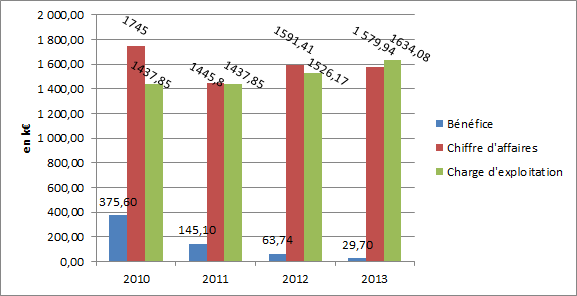
\includegraphics{compta.png}
\captionof{figure}{Comptabilité de Logilab sur les exercices comptables des trois dernières années}
\end{center}

\subsection{Position de Logilab sur le marché}
\paragraph{}
De nos jours, l'informatique est au cœur de toutes les entreprises. De nombreuses sociétés de services informatiques ont vu le jour ces dernières années. Les principaux concurrents de Logilab, sont de grandes SSII\footnotemark[3] comme Capgemini, Accenture, Logica, Atos ou Steria. Afin de se démarquer sur un marché saturé, Logilab a mis l'accent sur sa spécialisation dans les domaines scientifiques et sémantiques ainsi que dans le développement du langage Python. Toutefois, sa spécialisation dans le domaine de l'informatique scientifique et le Web sémantique ne leur permet d'apparaître que sur ce marché.

\footnotetext[1]{Le bénéfice d'une entreprise est la différence positive entre : d'une part la somme des recettes réelles (produits comptabilisés) et produits calculés (factures à émettre, charges comptabilisées d'avance) et d'autre part la somme des dépenses réelles (charges comptabilisées) et des coûts calculés (amortissements, provisions, factures à recevoir...)}
\footnotetext[2]{Le chiffre d'affaires d'une entreprise est le total des ventes d'une entreprise sur un exercice comptable}  
\footnotetext[3]{SSII : Société de service en ingénieurie informatique}

\paragraph{}
Logilab étant spécialisée dans le domaine scientifique et la gestion de données, l'entreprise possède de nombreux clients dans des domaines très divers comme : l'énergie, la télécommunication, les établissements publics, l'enseignement, l'aéronautique et l'espace. Ces principaux clients sont EDF, la BnF\footnotemark[1], l'IRSN\footnotemark[2], la SNCF, la  RATP, France Télécom R\&D, Bouygues Telecom, mais aussi des établissement publics comme le Ministère de l'Intérieur.

\footnotetext[1]{Bibliothèque nationale de France}
\footnotetext[2]{Institut de Radioprotection et de Sûreté Nucléaire}

    Logilab participe ainsi à des projets d'envergure comme par exemple :
\begin{itemize}
\item \url{http://data.bnf.fr/}
\item \url{http://brainomics.net/}
\item \url{http://collections.musees-haute-normandie.fr/collections/}
\end{itemize}

\subsection{Analyse des risques encourus par l'entreprise}
\paragraph{}
Comme la majorité des petites entreprises, il existe des risques inhérents à l'activité de Logilab, détaillés ci-après, liés aux produits, aux équipes et aux clients. La connaissance et la compréhension de ces risques sont essentielles afin de les maîtriser impérativement. Le risque majeur, concernant les produits de Logilab, serait l'incapacité à financer leur développement. Par ailleurs, le produit phare de Logilab CubicWeb ne possède pas une communauté propre importante. Or dans le monde des logiciels \textit{open source}, une forte communauté est un atout important. Logilab est composée d'une vingtaine de personnes, le départ d'une personne clé est donc un risque important pour le fonctionnement de l'entreprise. De plus, l'évolution de carrière étant limitée dans une entreprise de cette taille, les départs se renouvellent fréquemment. Il existe également un autre risque lié au pilotage des développeurs : les entreprises de logiciels \textit{open source} attirent des personnes qui adhèrent à une vision libertaire et peuvent avoir des difficultés à accepter le principe hiérarchique d'une entreprise, même si dans le contexte de Logilab la pression hiérarchique est faible. De part sa petite taille, l'existence de Logilab repose sur le financement de ses clients ; la perte de plusieurs clients ou encore une baisse de réputation qualité serait un risque majeur pour l'entreprise.


\chapter{Organisation générale}

\section{Organigramme et postes}

\begin{center}
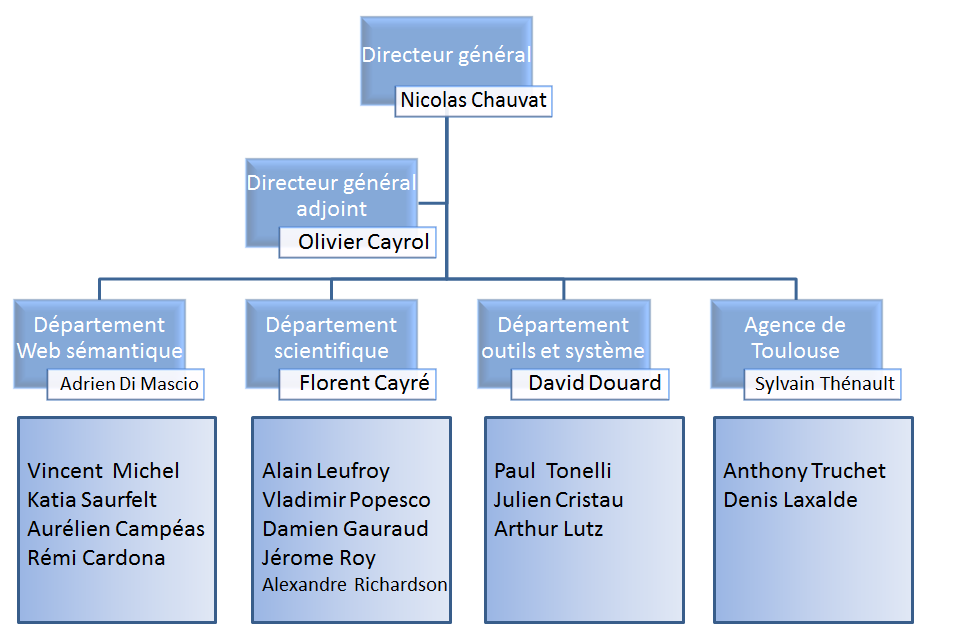
\includegraphics[scale=0.7]{organigramme.png}
\captionof{figure}{Organigramme de l'entreprise Logilab}
\end{center}



\paragraph{Organigramme et flexibilité}
Logilab est divisée en quatre départements, comme le montre la figure ci-dessous : le département Web sémantique (SEM), le département informatique scientifique (DIS), le département outils et système (DOS) et l'Agence de Toulouse, département transversal. Les départements ne sont pas hermétiques : les affections sur les projets priment sur la division en département afin d'acquérir une flexibilité maximum. Logilab a récemment ouvert un établissement à Toulouse qui comptent aujourd"hui trois personnes. Cette expansion de Logilab à Toulouse permet un rapprochement avec les clients de cette région.

\paragraph{Profil des employés}
Le profil des personnes recrutées est varié. En effet, les personnes travaillant dans l’entreprise sont toutes ingénieurs mais ont des formations scientifiques très diverses. On retrouve des personnes spécialisées dans les mathématiques, l’électronique, la mécanique, la physique des plasmas, le traitement du langage naturel, etc. Cette diversité des profils est capitale pour Logilab qui, étant spécialisée dans la vente de compétences et d’expertises, doit disposer d’interlocuteurs utilisant le même vocabulaire et maitrisant les mêmes concepts scientifiques que ses clients. 



\section{Le département Web sémantique}
\paragraph{}
La recherche est au cœur de Logilab afin de rester compétitive sur un marché en expansion. Chaque département intègre une section recherche. Ce stage, effectué au sein du département Web sémantique, s'inscrit dans cette démarche de recherche et d'amélioration interne. Les principaux projets réalisés par le département au cours de ce stage sont les projets data.bnf.fr, Fevis, Brainomics.

\subsection{La Bibliothèque nationale de France}
\paragraph{}
Le projet data.bnf.fr s'inscrit dans une démarche d'ouverture des données sur le Web. Afin d’encourager la réutilisation des données brutes, cette ouverture a un aspect technique, avec le respect des standards du « Web sémantique » et ouverture sur le « Web de données » définis par le W3C, et un aspect juridique. En effet, les données sont placées sous Licence ouverte de l’État autorisant la réutilisation libre, y compris commerciale, avec mention de la source. Les outils du « Web de données » répondent à des problèmes anciens des bibliothèques, en particulier autour de la gestion de formats divers et de l’échange de données. Ils offrent une présence nouvelle de ces ressources sur le Web en les rendant plus facilement accessibles, réutilisables et en les liant à des ressources complémentaires.


\subsection{Fevis}
\paragraph{}
Le projet Fevis est un projet pour la Fédération des Ensembles Vocaux et Instrumentaux Spécialisés. La particularité du projet repose sur une aide à la saisie et la création d'un moteur de recherche sur les compositeurs. 

\subsection{Brainomics}

\paragraph{}
Brainomics est un projet de recherche collaboratif financé en partie par l'ANR (Agence Nationale pour le Recherche) qui apporte des solutions méthodologiques et logicielles pour l'intégration de la neuro-imagerie et des données génomiques. La génomique est une discipline de la biologie moderne qui étudie le fonctionnement d'un organisme à l'échelle du génome. Les ensemble de données de la neuro-imagerie et génomiques contiennent un très grand nombre de données cliniques et génétiques. 

\paragraph{}
Ce projet a deux objectifs principaux :
\begin{itemize}
\item la création d'un outil de gestion de données issues de la neuro-imagerie (imagerie fonctionnelle et anatomique), de la génomique, et de la clinique (questionnaires comportementaux) ;
\item sa mise en œuvre sur des architectures d'algorithmes de fouille de données et d'apprentissage statistique pour ces données.
\end{itemize}

\paragraph{}
Le point fort de ce projet est l'accès aux informations pertinentes dans un grand nombres de données. En effet, le modèle de données est optimisé pour des grand volumes. Brainomics apporte donc une solution \textit{open source} pour gérer les bases de données d'imagerie cérébrale et méta-données associées. 



\section{Composition de l'équipe projet}
\paragraph{}
Chaque membre de Logilab prend part à un projet soit en tant que développeurs soit en tant que responsable soit les deux. La composition type d'une équipe de développement associée à un projet est la suivante : 
\begin{itemize}
\item un chef de projet, interlocuteur principal du client, responsable des livrables et du respect des délais.
\item un responsable qualité de Logilab, s’assure de la qualité des livrables
\item l’équipe en charge de la réalisation, composée de développeurs et d’experts, selon le profil du projet.
\end{itemize}

\paragraph{}
Les postes de développeur et de chef de projets ne sont pas exclusifs. Un chef de projet est également un développeur, qui peut travailler en parallèle sur un projet où il n’est pas chef de projet. Cela lui permet ainsi de mieux comprendre et appréhender les difficultés rencontrées par l'équipe de développement.





\part{Méthodologie de l'entreprise et organisation du travail}
\chapter{Gestion de projet}
\section{Méthode agile}
\paragraph{}
Une méthode agile fonctionne sur la base de l'itératif et de l’incrémental. Les tâches sont réalisées progressivement, par ordre de priorité, avec des  phases de contrôle et d’échange avec le client. Les méthodes agiles, plus pragmatiques que les méthodes traditionnelles,  impliquent au maximum le client ce qui permet une grande réactivité à ses demandes. Elles visent la satisfaction réelle du client, même si ce dernier n'a pas défini précisément ses attentes lors de la rédaction du contrat. En effet, ses attentes vont se préciser au cours de la réalisation du projet. Logilab privilégie les méthodes agiles pour ses clients et son développement interne. Toutefois, bien qu'elle soit spécialisée dans les méthodes agiles et offre même des formations à ce sujet, elle laisse le choix à ses clients entre une méthode de gestion de projet traditionnelle et une méthode agile. 
\paragraph{}
Les méthodes agiles présentent l’avantage de travailler sur des sous-projets, moins complexes que le système complet, de les intégrer au fur et à mesure et de valider régulièrement leur fonctionnement correct par rapport aux besoins et exigences des utilisateurs finaux. Le client suit donc l'évolution du projet et peut réorienter le projet à tout moment ce qui diminue le risque de non-satisfaction. La limite des méthodes agiles réside dans la disponibilité et l'engagement du client. Ce dernier doit être impliqué ; il doit effectuer des tests, rediriger les spécifications si nécessaire, tout au long du projet.

\paragraph{}
Dans le cadre de ce stage, les développements effectués visent à l'amélioration des outils de Logilab et donc appartiennent au développement interne. La méthode agile a donc été appliquée tout au long de ce stage. Cette méthode fut particulièrement efficace car elle représentait une sécurité pour garantir la satisfaction de mon tuteur et de la direction ainsi que pour garantir la réalisation du projet. 

\section{Procédures de développement du projet}
\paragraph{}
Le projet est découpé en itérations. Une itération dure environ deux semaines. Une itération comprend typiquement les étapes suivantes :

\begin{center}
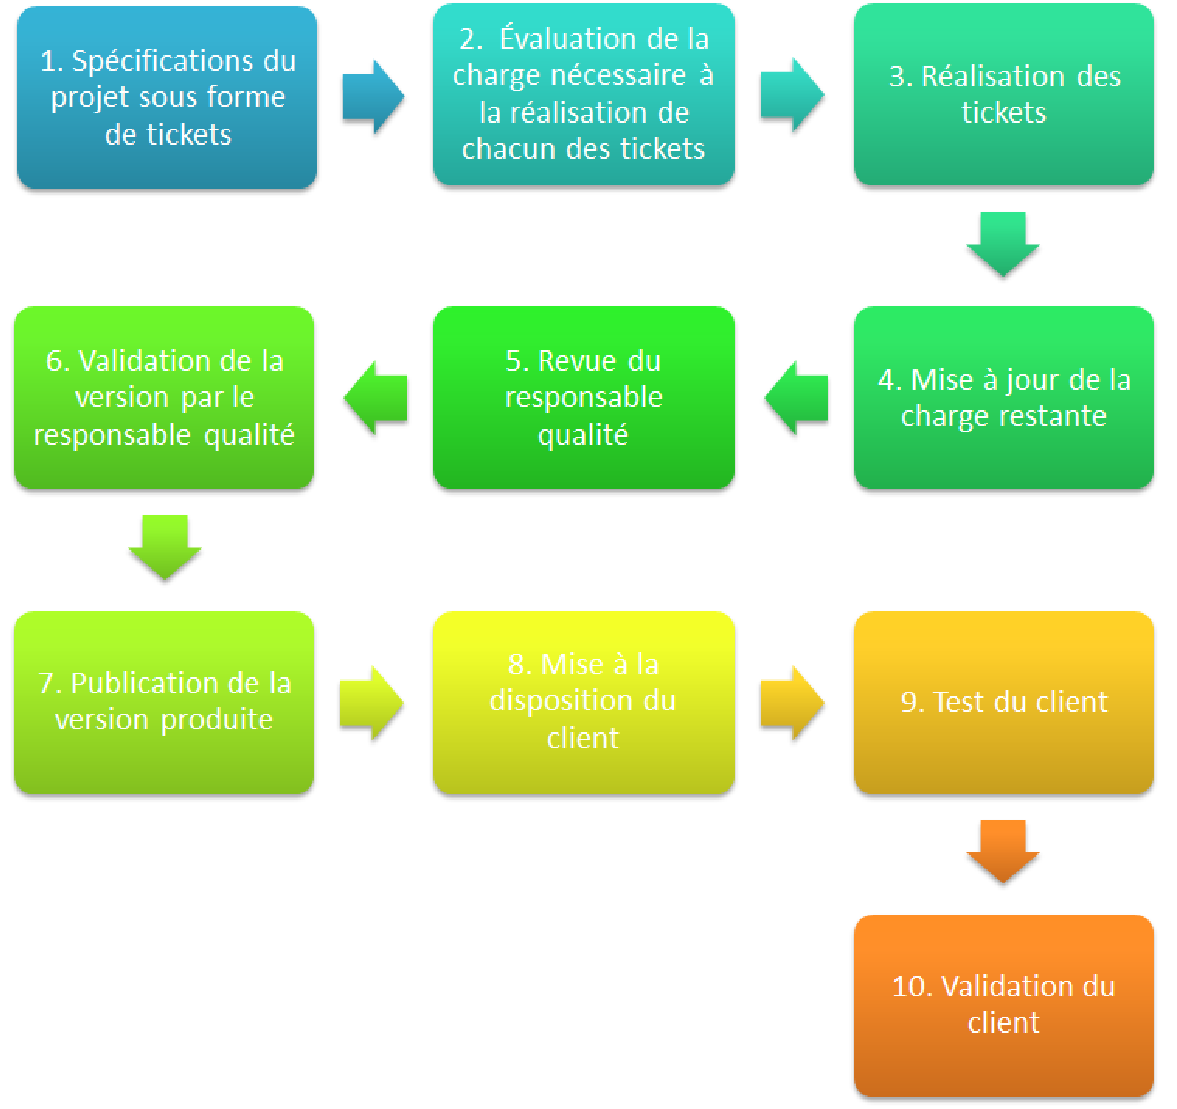
\includegraphics[scale=0.5]{iteration.png}
\captionof{figure}{Exemple d'itération d'un projet}
\end{center}

\paragraph{}
Le processus de développement permet de disposer d’une version fonctionnelle du projet à chaque fin d’itération. L'ordonnancement des tâches, le versionnement et la planification du développement sont explicités ci-après.



\paragraph{Ordonnancement des tâches}
Dans le contexte d'un projet client, l'itération des tâches est déduite du cahier des charges et se fait par l'élaboration de tickets, précisant la durée de la tâche, son importance et son statut. Un ticket est caractérisé par le nom de la personne qui traite le ticket, l'état du ticket, une description et des commentaires. Il peut avoir quatre états : \textit{en cours}, \textit{ouvert}, \textit{fait} ou \textit{en attente de retour}. La description du ticket reflète le besoin du client. Il est mis à jour si le besoin évolue ou s'il est précisé. Sur chaque ticket, un mécanisme de commentaires permet un dialogue entre Logilab et le client (demandes de précisions, alternatives techniques, compléments d’information, etc.) De plus, la charge de réalisation de chaque ticket (en jours.hommes) est évaluée par les personnes susceptibles de le réaliser afin d'être la plus réelle possible. Travaillant dans le cadre d'un projet interne, l'élaboration des tickets décrivant les travaux que je devais réaliser a été directement faite par mon tuteur. La version du projet est construite à partir de ces tickets. L'ordonnancement des tâches par des tickets apporte dynamisme et flexibilité.



\paragraph{Version et livraison}
Dans le cadre d'une méthode agile, chaque projet est découpé en versions, livrées régulièrement au cours du projet. Les versions du projet peuvent être \textit{"prévues"}, \textit{"en cours de réalisation"}, \textit{"livrées"}, ou \textit{"recettées"}. La procédure de développement d'une version est explicitée par des tickets qui indiquent les différentes tâches à effectuer. Avant chaque livraison, la version est testée de manière approfondie. La version qui est livrée est clairement identifiée comme telle dans le gestionnaire de version Mercurial, contenant le code source. Les caractéristiques de cet outil essentiel seront détaillées ultérieurement (Cf paragraphe 5.2.1). De plus, chaque livrable est accompagné de rapports qui identifient les tests unitaires qui échouent. Un test unitaire vérifie, sur un morceau de code précis, qu'un exemple particulier de la problématique, couvert par le test, a le comportement attendu. La validation d’une version d’un projet aboutit à sa publication. Il existe un entrepôt public pour les logiciels libres publiés par Logilab, un entrepôt sécurisé pour les logiciels développés en interne, et des entrepôts sécurisés pour chaque client. L'ensemble de mon code source a donc été déposé dans l'entrepôt sécurisé consacré aux projets internes.

\section{Contrôle et échange avec le client}
\paragraph{}
Dans un projet suivant une méthode agile, l'implication du client conditionne la réussite du projet. Les clients doivent donc être disponibles pour définir les versions et les tickets, pour tester les versions livrées et effectuer un travail de spécification tout au long du projet. Dans le contexte du stage, le projet étant un projet interne, la direction était très impliquée et disponible.
\paragraph{}
Dans le cadre d'un projet client, toutes les deux semaines environ une version préliminaire du projet est livrée afin d'obtenir le retour du client. Il peut alors préciser son besoin et échanger sur le travail rendu. Cela permet de garantir qu'il est satisfait du travail rendu. Dans le cadre de ce stage, chaque ticket était validé par le tuteur et chaque livraison était suivie d'une réunion avec la direction pour établir la suite du projet en fonction des attentes et de la réalisation. Cela a permis de visionner l'avancement du travail et de rediriger le projet au moment voulu.
\paragraph{}
La direction, comme les clients de Logilab, a eu la possibilité de suivre de façon précise l’avancée des travaux à travers le gestionnaire de sources contenant le code source et à travers l’extranet. L’extranet contient la description de l’ensemble des versions du logiciel et de leur état d’avancement. Il constitue une photographie précise et toujours d’actualité du projet et de son avancement. Les anomalies éventuelles peuvent être rapportées sur l’extranet. Une nouvelle version qui contient la correction d’une ou plusieurs des anomalies signalées peut alors être définie.



\chapter{Plan Qualité}
\section{Objectifs qualité}
\paragraph{}
Les objectifs qualité concernent tous les aspects du service fourni au client et visent à satisfaire ses besoins sur les plans de l’exploitation, de la maintenance et de l’assistance à l’utilisation. À chaque besoin correspond des exigences nécessaires à l’assurance de la qualité. Ainsi concernant l'exploitation, Logilab s'engage à fournir une adéquation fonctionnelle, une stabilité de la version, une facilité de maintenance et une disponibilité pour l'assistance à l'utilisation.
\section{Mise en œuvre du plan Qualité}
\paragraph{}
Pour respecter ces exigences, Logilab assure la traçabilité et conserve un historique des événements et des actions, conçoit des systèmes modulaires réutilisables, teste tous les livrables et développe les compétences des équipes, à travers des formations, des conférences et du travail en groupe.
\subsection{Traçabilité et conception modulaire}
\paragraph{}
Pour assurer la traçabilité, Logilab utilise des outils et systèmes  qui permettront de conserver un historique des actions de développement (gestion de versions),  des actions de déploiement (gestion de configuration) et de documentations et de dialogues entre partenaires du projet (gestion des connaissances). Cette traçabilité permet de résoudre plus rapidement une anomalie et de savoir si elle a déjà été rencontrée. La conception modulaire facilite le remplacement et l’évolution des composants, ainsi que la répartition des responsabilités, que ce soit entre les sous-systèmes ou au sein de l’architecture globale. 
\subsection{Tests}
\paragraph{}
Tous les éléments et livrables produits sont testés avec des jeux d’essai validés par le client et passés en revue pour garantir qu’ils correspondent à leurs spécifications. Ces validations seront appliquées tant à la documentation, qu’au déploiement des systèmes ou aux logiciels. Dans le cas des logiciels, Logilab utilise des outils d’analyse statique de code, des outils de couverture de test, et des plateformes de tests automatiques effectuant des tests unitaires, des tests d’intégration et des tests de non-régression. Toutes les nuits, un outil de test automatique récupère, dans l’outil de gestion des sources, la version du projet en cours de développement puis va effectuer une série de tests permettant de s’assurer de la qualité: 
\begin{itemize}
\item lancement automatique des tests disponibles dans le projet (tests unitaires et tests d’intégration),
\item calcul de la couverture de test,
\item production automatique de la documentation,
\item production automatique des éléments déployables (par exemple les paquets binaires installables). 
\end{itemize}
    Le résultat de cette série de tests est disponible dans l’extranet.
\subsection{Accroissement des compétences}
\paragraph{Formations} Le maintien ou l’accroissement des compétences des équipes impliquées dans le projet permet d’assurer un suivi de la qualité dans le temps. Les membres du personnel peuvent ainsi s'inscrire à des formations comme celles dédiées au management ou à Hadoop\footnotemark[1].
\paragraph{Vsprint}
Le vsprint correspond à une plage horaire hebdomadaire (les vendredi après-midi) où chaque membre du personnel est affecté par son directeur de département à un binôme et doit travailler sur un ensemble de tickets, généralement lié au développement d'outils internes. L'objectif est de partager les bonnes pratiques de développement, de faire connaître les projets, de mutualiser le code et les idées et d'améliorer de façon continue les outils internes à l'entreprise. Cette pratique est pertinente car elle permet de diffuser la connaissance entre les développeurs et d'imposer une plage horaire pour le développement des outils de l'entreprise afin qu'elle reste compétitive.


\footnotetext[1]{Hadoop est un framework Java libre destiné à faciliter la création d'applications distribuées et échelonnables. Il permet aux applications de travailler avec des milliers de nœuds et des pétaoctets de données.}

\section{Bilan et retours d'expérience d'un projet}
\paragraph{}
Chaque fin de projet est l’occasion d’effectuer un bilan et de dégager des pistes d’amélioration de la méthode de travail et du plan qualité. La pertinence de ces pistes d’amélioration est jugée par le responsable qualité de Logilab et un groupe de travail dédié. Les pistes retenues sont immédiatement mises en application. Le plan qualité et la méthode de travail font donc tous deux l’objet d’améliorations constantes directement issues des retours d’expérience.

\chapter{Outils utilisés}
\section{Cubicweb}
\subsection{Les valeurs ajoutés de CubicWeb}
\paragraph{}
CubicWeb est une plateforme logicielle libre implémentée par l'entreprise Logilab et à la base de la majorité de leurs applications ; il m'a donc été amené à utiliser ce framework\footnotemark[1] quotidiennement.



\paragraph{Des composants assemblables et adaptables}
La plateforme CubicWeb est composée de fonctionnalités préprogrammées, développées en Python, appelées "cubes". Ces "cubes" adaptables sont assemblables et permettent de construire des applications facilement et rapidement. De cette manière, elle permet aux développeurs de se concentrer sur les spécificités de leur application plutôt que d'avoir à réinventer les briques essentielles de l'import, la fusion, la publication, l'interrogation et la visualisation de données. 
\paragraph{Prototypage rapide}
La plateforme permet de développer rapidement des applications de gestion de données. En effet, le développeur dispose de fonctionnalités automatisant, à partir du modèle des informations, les tâches habituelles comme la gestion de la base relationnelle sous-jacente, la génération d'une interface Web par défaut et la migration entre versions successives. Cette technique de réutilisation de code améliore considérablement le temps de production d'application Web et permet un prototypage rapide permettant de répondre aux critères des méthodes agiles.

\paragraph{Une plateforme centrée sur les données}
L'avènement du Web sémantique et de l'Open Data\footnotemark[2] nécessite de disposer d'outils adaptés pour développer des applications centrées sur les données. \textit{CubicWeb} place les données au cœur du système en offrant la possibilité d'importer des données facilement, de les mettre en relation lorsqu'elles proviennent de sources disjointes, de les republier et de faciliter leur interrogation et leur visualisation. 

\footnotetext[1]{framework : ensemble de composants logiciels permettant de créer l'architecture d'un logiciel}
\footnotetext[2]{Open data : données diffusées de manière structurée selon une méthodologie et une licence ouverte garantissant son libre accès et sa réutilisation par tous, sans restriction technique, juridique ou financière.}

\paragraph{Une liberté pour le client}
CubicWeb s'appuie sur le modèle métier des informations gérées qui laisse à l'utilisateur la possibilité de naviguer dans le graphe des informations, de sélectionner des données et de choisir la vue qui lui permettra de les visualiser.





\paragraph{Respect des standards ouverts d'Internet}
CubicWeb respecte les standards ouverts d'Internet afin de simplifier les communications et les échanges. Elle suit les standards du W3C\footnotemark[1] (RDF\footnotemark[2], SPARQL\footnotemark[3], HTML5\footnotemark[4], CSS3\footnotemark[5], Responsive Design\footnotemark[6]) et peut gérer nativement plusieurs modèles de données faisant office de standards de faits (FOAF\footnotemark[7], SIOC\footnotemark[8], DOAP\footnotemark[9]).

\footnotetext[1]{W3C (World Wide Web Consortium) est un organisme de normalisation à but non lucratif chargé de promouvoir la compatibilité des technologies}

\footnotetext[2]{RDF (Resource Description Framework) est un modèle de graphe destiné à décrire de façon formelle les ressources Web et leurs métadonnées, de façon à permettre le traitement automatique de ces descriptions. }

\footnotetext[3]{SPARQL est un langage de requêtes et un protocole qui permet de rechercher, d'ajouter, de modifier ou de supprimer des données RDF disponibles à travers Internet.}

\footnotetext[4]{HTML5 est la cinquième version du format de données HTML conçu pour représenter les pages Web}

\footnotetext[5]{CSS3 est un langage servant à décrire la présentation des documents HTML et XML.}

\footnotetext[6]{Responsive Design est une notion de conception de sites Web qui permet à l'utilisateur de consulter le même site Web à travers une large gamme d'appareils (moniteurs d'ordinateur, smartphones, tablettes, TV, etc.) avec le même confort visuel.}

\footnotetext[7]{FOAF est un vocabulaire RDF permettant de décrire des personnes et les relations qu’elles entretiennent entre elles. C'est une application du Web sémantique.}

\footnotetext[8]{SIOC est un vocabulaire utilisant RDF permettant de décrire des objets couramment utilisés sur les sites communautaires et leurs relations. SIOC est une application du Web sémantique pour décrire des blogs, des forums, des wikis... }

\footnotetext[9]{DOAP est un vocabulaire RDF décrivant les projets logiciels}


\subsection{Architecture générale de CubicWeb}

\paragraph{}
L'architecture de CubicWeb sépare clairement la partie dédiée au client (\textit{Web engine}) et l'entrepôt des données.  Elle est représenté par la figure suivante:

\begin{center}
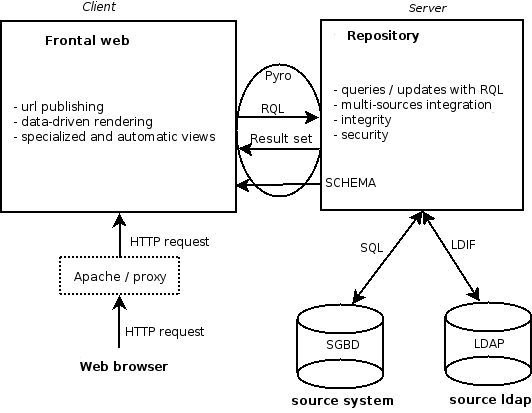
\includegraphics[scale=0.7]{archi_globale.png}
\captionof{figure}{Schéma de l'architecture de CubicWeb}
\end{center}

\paragraph{L'entrepôt de données}
L'entrepôt de données encapsule et assemble un accès à une ou plusieurs sources de données : données SQL, annuaires LDAP, autres applications de CubicWeb, systèmes de fichiers etc. Toutes les interactions avec l'entrepôt de données sont effectuées en utilisant le langage \textit{Relation Query Language}, que nous développerons ultérieurement. Il fédère les sources de données. L'émetteur de la requête ignore si une requête s'étend sur plusieurs sources de données ou nécessite l'exécution des sous-requêtes. Cette séparation entre l'entrepôt de données et l'interface utilisateur simplifie l'écriture de la requête pour l'utilisateur et permet de cacher la complexité du multisource.

\paragraph{Modélisation des données}
Les données des applications de CubicWeb sont modélisées suivant un schéma. Le module python \textit{Yams}, qui signifie \textit{Yet Another Magic Schema}, définit le schéma générique des relations et des entités de manière simple et générique. Une entité est un objet qui continet une séquence d'attributs, un identifiant (\textit{eid}) et des relations. Un type de relation est utilisé pour définir une relation binaire orientée entre les types d'entité . La partie gauche d'une relation est nommée le sujet et la partie droite est nommée l'objet. Une définition de relation est un triplet (type de sujet de l'entité, type de relation, type d'entité de l'objet) associé à un ensemble de propriétés telles que la cardinalité, les contraintes, etc.

\paragraph{}
Les données de l'application sont ensuite modélisées suivant un schéma entités-relations, où chaque entité ou relation hérite du modèle correspondant dans \textit{Yams}. Cette modélisation des données se trouve dans un composant de CubicWeb appelé "cube" (Cf paragraphe 5.1.3) L'exemple ci-dessous modélise l'organisation de projet :

\renewcommand{\lstlistingname}{Exemple}
\begin{lstlisting}[caption= Schéma de l'organisation d'un projet]
class Projet(EntityDefinition):
	nom : String()
	domaine : String()
	duree : int()

class Personne(EntityDefinition):
	nom : String()
	personne : String()
	
class responsable_de(RelationDefinition)
	subject : Personne
	object : Projet
\end{lstlisting}

\paragraph{Requêtes RQL}
RQL est le langage informatique d'exploitation de bases de données, utilisé par \textit{CubicWeb}. Grâce à une syntaxe de haut niveau, il permet d'accéder aux données stockées dans les bases de données et d'explorer les entités, attributs, relations du schéma très facilement. RQL utilise un solveur pour automatiquement déterminer les types possibles pour une variable en fonction du modèle de données et des contraintes exprimées dans la requête. Il se base sur le concept de relation binaire ordonnée : <subject> <relation> <object> . Voici ci-dessous différents exemples de requêtes retournant respectivement: les 10 derniers projets créés, les projets commençant par C, et le nombre de personne responsable d'un projet.

\renewcommand{\lstlistingname}{Exemple}
\begin{lstlisting}[caption= Requêtes RQL]
Any X ORDERBY XD DESC LIMIT 10 WHERE X creation_date XD, X is Projet
Any X WHERE X is Projet, X name LIKE 'C%'
Any X,COUNT(P) GROUPBY X WHERE P responsable_de X
\end{lstlisting}

\paragraph{}
    Une requête retourne un \textit{ResultSet} qui est un tableau à deux dimensions (liste de listes) où le nombre de lignes correspond au nombre de résultats et le nombre de colonnes correspond au nombre d'éléments sélectionnés dans la requête. La classe \textit{ResultSet} expose, en plus d’une interface de tuple, les principaux attributs et fonctions suivants :
\begin{itemize}
\item description : description du résultat sous forme de liste de listes,
\item entities() : itère sur les entités pour une colonne donnée,
\item get\_entity() : renvoie l’entité pour une ligne et une colonne
données.
\end{itemize}

\paragraph{}
Dans CubicWeb, les requêtes RQL sont définies sous forme d'un graphe où chaque nœud peut être une variable, une constante, une condition d'existence ou une relation. Il existe quatre types d'arbre de requêtes RQL répondant aux fonctionnalités classiques d'un langage de requête : sélection, modification, supression, insertion. Soit la requête suivante, composée de trois unions, une condition d'existence et d'une sous-requête : 
\begin{lstlisting}[caption= Requête RQL]
(Any X WHERE X relation Y) 
UNION (Any X WHERE X relation Y, EXISTS(X name A))
UNION Any X WHERE X relation Y WITH X,Y BEING (Any A,B WHERE A name B))
\end{lstlisting}

Sous forme d'arbre elle s'écrit ainsi:
\begin{center}
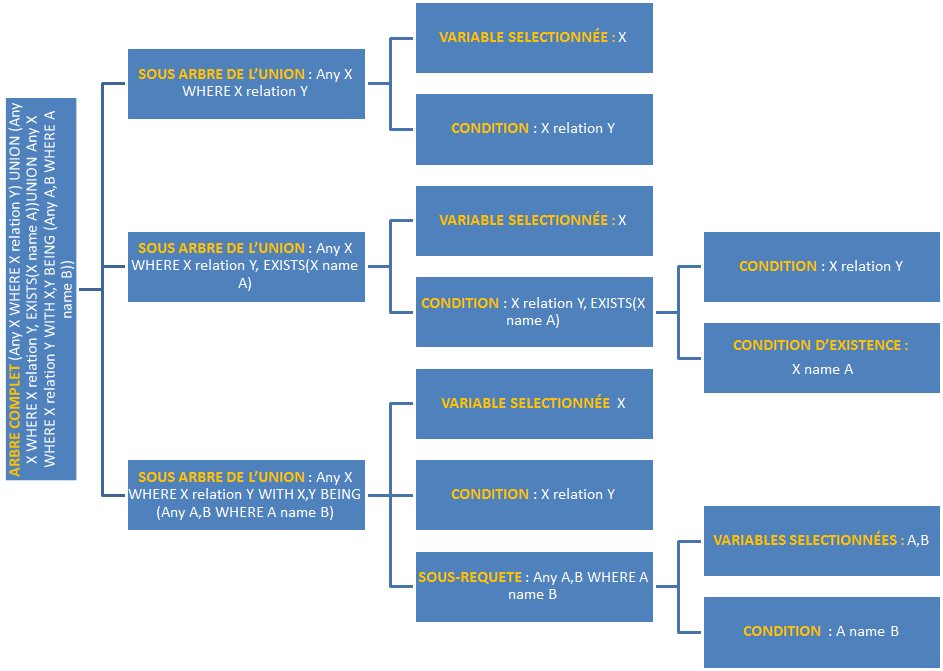
\includegraphics[scale=0.7]{graph.png}
\captionof{figure}{Exemple de graphe d'une requête RQL}
\end{center}

\paragraph{}
Le module python \verb+rql+ contient un analyseur et des fonctions utilitaires pour manipuler l'arbre de syntaxe de la requête. On a alors accès à différentes méthodes qui permettent par exemple d'ajouter des nœuds, des relations, des sous-requêtes etc.


\paragraph{Génération de tables SQL}
Les tables SQL sont générées automatiquement par Yams à partir du modèle de données décrit dans CubicWeb.

\paragraph{Web engine}
Le moteur Web répond à des requêtes HTTP et construit l'interface utilisateur. Par défaut, le moteur Web fournit une interface utilisateur sur la base du modèle de données de l'instance. Les entités peuvent être créées, affichées, mises à jour et supprimées. 

\subsection{Le cube}
\paragraph{}
Un \textbf{cube} est le composant logiciel de base de CubicWeb, comportant trois parties principales : le modèle de données \textit{(schema)}, la logique métier \textit{(entities)}, l’interface utilisateur \textit{(views)}, ainsi que des dépendances vers d’autres cubes. On peut distinguer deux types de cube : un cube métier qui définit un schéma et une logique propre à un concept métier particulier (cube \textit{file} pour la gestion des fichiers, \textit{person} pour la modélisation du concept de personne, etc) et un cube applicatif qui définit la logique nécessaire à une application complète, en s'appuyant sur un certain nombres d’autres cubes (métiers).
    \begin{center}
    L’infrastructure de base d’un cube est : \\
    \end{center}
\begin{tabular}{|l|l|}
\hline
data/ & stocke les données Web (CSS, JS, images)\\
debian/ & comprend les informations pour la construction de paquets Debian\\
entities.py &\\
i18n/ & comprend les fichiers .po pour l'internationalisation du cube (français, anglais, espagnol...)\\
migration/ & contient les fichiers de migration et \\
           & le code qui sera exécuté après l'initialisation de la base de données\\
\_\_pkginfo\_\_.py & contient les méta-données du cube et les dépendances vers les autres cubes\\
hooks.py & fichier permettant la gestion d'évènements (comme la suppression d'une entité par exemple)\\
setup.py & fichier pour la distribution et l'installation du cube\\
schema.py & définit le modèle de données\\
test/ & comprend les tests du cube\\
views.py & définit les vues de l'interface propre au cube\\
uiprops.py & indique les fichiers css et javascript à prendre en compte pour la mise en forme\\
\hline
\end{tabular}

\paragraph{Création et lancement d'une instance}
Dans la plateforme CubicWeb, pour créer une instance, la commande \verb+cubicweb-ctl create <nom-cube> <nom-instance>+ permet de créer une instance. La commande \verb+cubicweb-ctl start <nom-cube> <nom-instance>+ permet de lancer une instance. La création de l'instance du cube crée donc une application avec l'architecture par défaut.

\paragraph{Gestion d'évènements}
Les \textit{hooks} sont des traitements à effectuer lorsque certains événements se produisent dans une application CubicWeb. Ils servent en particulier à ajouter un ensemble de contraintes ne pouvant
être exprimées dans le schéma, ou permettre le calcul automatique d’un attribut ou d’une relation (e.g. à l’insertion ou la mise à jour d’une entité). Les évènement sur les données sont créées par des \textit{hooks} mais ne sont exécutées qu'au \verb+commit+ ou au rollback d'une \verb+transaction+. Ils se sélectionnent sur un ensemble des évènements suivants:
\begin{itemize}
\item \textbf{Évènements du serveur} :
    \begin{itemize}
    \item démarrage ou arrêt du serveur,
    \item ouverture ou fermeture de session.
    \end{itemize}
\item \textbf{Évènements sur les données} :
    \begin{itemize}
    \item avant ou après la création d’une entité
    \item avant ou après la mise à jour d’une entité
    \item avant ou après la suppression d’une entité
    \item avant ou après l’ajout d'une relation
    \item avant ou après la suppression d’une relation 
    \end{itemize}
\end{itemize}




\section{Autres outils techniques}
\subsection{Mercurial : gestionnaire de version}
\paragraph{}
Mercurial est un logiciel de gestion de versions décentralisé qui administre les différentes versions d'un programme écrites par un ou plusieurs développeurs. Il conserve l’historique des modifications, permet de paralléliser des réalisations puis de les intègrer, et met en place des drapeaux marquant les versions publiées en fin d’itération. Dans un contexte de développement de logiciel en équipe et dynamique dans le temps, maintenir un ensemble de versions est indispensable pour l'aboutissement du projet. Mercurial permet la gestion avancée de l’historique des modifications dans un environnement distribué (plusieurs contributeurs). Il gère aussi bien le code source des éléments logiciels que la documentation du projet. La gestion de versions décentralisée consiste à voir l'outil de gestion de versions comme un outil permettant à chacun de travailler à son rythme, de façon désynchronisée des autres, puis d'offrir un moyen à ces développeurs de s'échanger leur travaux respectifs. De fait, il existe plusieurs dépôts pour un même logiciel. Ce système est très utilisé par les logiciels libres. Cet outil, utilisé quotidiennement tout au long de ces vingt-quatre semaines, est indispensable pour le plan qualité du code.


\subsection{Python : langage de programmation}
\paragraph{}
Logilab a choisi de se spécialiser dans le langage de programmation Python car il présente de nombreux avantages comme la compacité, l'expressivité, la richesse de la bibliothèque standard et la portabilité de l’interpréteur. Tous ces avantages facilitent l’écriture d'un code logiciel maintenable et modulaire. Lors de ce stage, l'ensemble de mes implémentations a donc été écrites en Python.
\subsection{Debian GNU Linux}
\paragraph{}
Les solutions développées s'intègrent avec la distribution Debian GNU/Linux. De part son aspect non commercial et sa constitution uniquement en logiciel \textit{open source}, le choix de cette distribution de Linux est en parfaite adéquation avec la vision de l'entreprise. De plus, elle est facile à administrer et à déployer sur de grands parcs informatiques.

\subsection{Entrepôt de l'extranet}
\paragraph{}
Le projet est accessible au client par un extranet sécurisé \url{http://hg.logilab.fr/master/clients/}.  Dans un espace sécurisé, le site extranet contient chacun des projets menés avec le client. On y trouve les indicateurs et les informations nécessaires à la gestion du projet, comme l’avancement et la planification de la charge, les délais et le budget ; ainsi que les documents échangés comme les spécifications, les rapports d’anomalies et les demandes d’évolutions.
\paragraph{}
Le site extranet de gestion de projets mis en place par Logilab joue un rôle central dans le processus de travail et les relations avec le client. S’appuyant sur CubicWeb, il permet, outre les échanges d’informations, de conserver un historique complet du projet car il conserve toutes les dates de création et de changement d’états pour tous ces éléments. Le site extranet permet d’accéder à l’outil de gestion des sources et au répertoire de publication. Il est ainsi possible de récupérer le code en cours de développement, de naviguer dans ce code au travers d’une vue Web, de récupérer les différentes versions des documents publiés ou les différentes versions des éléments déployables (paquets binaires installables). Enfin, sur le site extranet, sont mis à disposition tous les documents échangés dans le cadre du projet : rapports, spécifications, comptes-rendus de réunions, etc. On y trouvera également le nom et les coordonnées des différents acteurs.
\paragraph{}
Ainsi l'extranet permet, d'une part, de juger des priorités et mieux maîtriser les risques, et d'autre part, de garantir la traçabilité des requêtes, la gestion des incidents et du suivi du projet dans son ensemble. Il propose une approche de la conduite de projet qui favorise la collaboration entre les parties et prône la transparence des travaux.



\section{Outils de communication et planification interne}
\subsection{Forum}
\paragraph{}
Outre les rencontres réelles au cours de réunions ou d’ateliers, Logilab met à disposition un ensemble de forums permettant aux développeurs de communiquer rapidement en cas de besoin et de tenir des réunions de travail, sans que leur localisation précise soit un obstacle (télétravail, résolution collaborative d’un problème rencontré sur un site client, support aux partenaires, etc.). Cinq forums constituent les canaux de communication internes et permettent une communication continue par thème (direction, développement,  informatique scientifique, gestion de connaissances, gestion du système informatique).
\subsection{Points d'avancement}
\paragraph{Synthèse hebdomadaire}
Chaque lundi, le personnel envoie un compte-rendu par courriel à l'ensemble des développeurs. L'objectif est d'identifier rapidement les dysfonctionnements possibles. L'avantage de compte-rendu par courrier électronique est que le temps est plus optimisé qu'en planifiant des réunions. Les inconvénients sont que ces comptes-rendus ne sont pas lus de tous ni rédigés de façon systématique le lundi mais peuvent être reportés dans la semaine. L'information circule plus difficilement. Le contenu type d'un compte-rendu se compose du travail effectué la semaine précédente, celui prévu pour la semaine en cours, les difficultés rencontrées et nécessitant de l'aide immédiate et un retour sur le Vsprint (Cf paragraphe 4.2.3)
\paragraph{Réunion mensuelle par département}
Une fois par mois, chaque département se réunit pour analyser les résultats, communiquer sur les projets en cours et signaler tout dysfonctionnement éventuel.
\subsection{Outil de planification du travail : JPL}
\paragraph{}
JPL est une application \textit{CubicWeb} qui permet de planifier le développement. L'équipe en charge du développement crée des versions non datées pour signaler les corrections et ajouts prévus. La date d'une version est déterminée par le client. En fonction du budget (en jours.hommes) attribué à Logilab par le client, des tickets peuvent être ajoutés ou retirés d'une version.





\part{Déroulement du stage}
\chapter{Le sujet}
\section{Problématique}
\paragraph{}
Les applications du Web Sémantique, telles celles développées sur la plateforme \textit{CubicWeb}, contiennent généralement d'importantes quantités de données hétérogènes, souvent issues de sources différentes. Une importante valeur ajoutée réside dans la capacité à traiter ces grands volumes de données pour en extraire des informations pertinentes. Une des solutions envisagée est de traiter les prédicats contenus dans les données avec des règles logiques visant à produire de nouveaux prédicats. Ce type de traitements fait appel à un moteur d'inférences. L'objectif des travaux est donc, à terme, d'offrir aux développeurs et aux utilisateurs d'une application \textit{CubicWeb}, la possibilité de traiter l'ensemble des données avec des règles en vue d'en extraire des nouvelles informations pertinentes. Mon stage vise donc à améliorer la plateforme \textit{CubicWeb}, utilisée dans tous les projets clients.


\section{Un sujet innovant et prospectif}
\paragraph{}
Le choix de ce stage fut motivé par la qualité innovante du sujet. Ce projet de mise en place de moteur d'inférences fait appel à la programmation logique, enseignée à l'Université de Technologie de Compiègne (UTC), mais encore très peu utilisée dans le monde industriel. Les enseignements de l'UTC IA01\footnotemark[1] et IA02\footnotemark[2] m'ont fait découvrir la  représentation des connaissances, le Web sémantique et la programmation logique. Étant très intéressée par l'ingénierie des connaissances et système d'information, ce stage, sous la tutelle d'un ingénieur spécialiste de la gestion de données, et portant sur les moteurs d'inférence, s'inscrit parfaitement dans mon projet professionnel et ma spécialisation future en filière ICSI.
\paragraph{}
Cette volonté de mettre en place des mécanismes intelligents dans des applications Web reste néanmoins un sujet prospectif. La recherche de solutions d'implémentation dans un contexte précis faisant partie du rôle de l'ingénieur, ce sujet ouvre des perspectives dans tous les projets clients à venir car elle améliore la plateforme CubicWeb.

\footnotetext[1]{Intelligence artificielle - représentation des connaissances}
\footnotetext[2]{Logique et résolution de problèmes par recherche}

\section{Rôle prédéfini et rôle réel}
\paragraph{}
L'intitulé du stage défini avant mon arrivé était : "Intégrée à l'équipe de recherche et développement "Web Sémantique" de Logilab, sous la tutelle de Vincent Michel, ingénieur spécialiste de la gestion de données, le rôle est de l'assister dans son travail quotidien et effectuer tout ou partie des travaux suivants, en collaboration avec l'équipe : étudier différents moteurs d'inférences utilisés dans le monde du Web Sémantique, intégrer un de ces moteurs dans la plateforme CubicWeb, tester le moteur sur une ou plusieurs applications existantes. Le sujet de mon stage a bien été respecté puisque j'ai effectivement travaillé sur la mise en place de moteur d'inférences dans \textit{CubicWeb}. Toutefois, la partie collaborative fut limitée. En effet, excepté lors des Vsprints (Cf paragraphe 4.2.3) , j'ai essentiellement cherché des solutions et des implémentations seule, présentées à ma hiérarchie et modifiées suivant les différents retours. Ce contexte m'a permis m'a permis de prendre de l'autonomie.


\chapter{Analyse du besoin réel et études}
\section{Les objectifs attendus}
\paragraph{}
La première partie de ce stage fut de comprendre les enjeux et les problématiques de la mise en place d'un moteur d'inférences dans la plateforme CubicWeb ; puis d'étudier les options possibles pour mettre en place le moteur d'inférences. Cette analyse a conduit à l'étude de nombreuses thèses en anglais et à la publication en interne d'une série de dossiers en français et en anglais, l'anglais étant privilégié.
\paragraph{}
Les objectifs réels de la mise en place des moteurs d'inférence dans la plateforme \textit{CubicWeb} sont de réduire le temps d'exécution des requêtes RQL et d'offrir aux utilisateurs la possibilité de traiter des ensemble de données via un comportement intelligent. Au cours de l'avancée de ce stage, de nouvelles applications possibles aux inférences se sont ajoutées :
\begin{itemize}
\item inférer les fermetures transitives
\item inférer sur les relations ternaires
\item apporter de la programmation logique aux attributs calculés pour améliorer le temps d'exécution des requêtes
\item améliorer les mécanismes de propagation des permissions dans une application.
\item simplifier à l'utilisateur l'écriture de requêtes complexes.
\end{itemize}

\section{Les options évaluées}
\paragraph{}
Concernant la simplification de l'écriture des requêtes, l'option envisagée est d'établir des règles simples au moyen de Python, dans un premier temps, et un mécanisme de réécriture, dans un second temps. Ce cas d'application de mise en place d'inférence est traité ultérieurement dans ce rapport. Pour mettre en place des inférences plus complexes que dans le cas d'application de la réécriture, plusieurs outils sont possibles : les \textit{reasoner} (solution proposée par l'équipe à mon arrivée), les systèmes experts (solution que j'ai ensuite proposée), les bases de données déductives (dernière option évaluée).

\footnotetext[1]{Une ontologie est l'ensemble structuré des termes et concepts représentant le sens d'un champ d'informations. L'ontologie constitue en soi un modèle de données représentatif d'un ensemble de concepts dans un domaine, ainsi que des relations entre ces concepts.}

\subsection{Reasoners}
\paragraph{Rôle d'un reasoner}
Un \textit{reasoner} est un programme capable d'inférer des conséquences logiques à partir de faits et d'axiomes et de vérifier qu'une ontologie\footnotemark[1] est cohérente. Pour vérifier la cohérence d'une ontologie, un \textit{reasoner} vérifie : 
\begin{itemize}
\item la généralité d'un concept : un concept ne doit pas englober un autre concept
\item si la définition d'un concept est instanciable
\item s'il n'y a pas de contradiction entre les axiomes et les relations
\item la cohérence du vocabulaire de l'ontologie.
\item déduire des relations
\end{itemize}
\paragraph{Fonctionnement d'un reasoner}
Pour parvenir à établir la cohérence d'une ontologie, les \textit{Reasoner} suivent le processus décrit dans la figure ci-dessous (Cf figure XXX).
\begin{multicols}{2}
\begin{center}
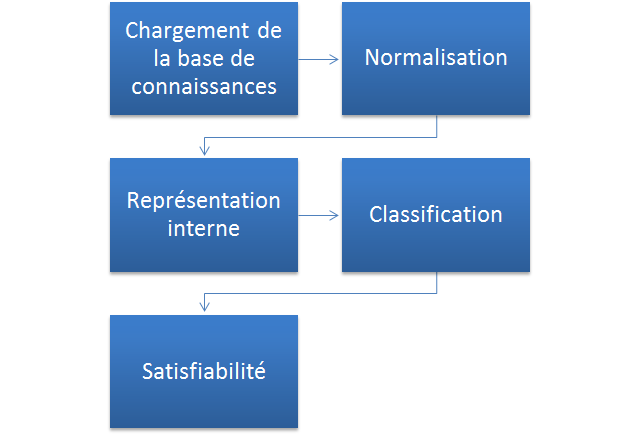
\includegraphics[scale=0.5]{process_reasoner.png}
\captionof{figure}{Processus de fonctionnement d'un reasoner}
\end{center}

\paragraph{Normalisation} Tous les concepts sont transformés sous une forme normalisée où seulement les opérateurs de négations, conjonction, restriction universelle XXX et le symbole XXX sont autorisés. De plus, les constantes sont éliminées ainsi que les doubles négations. Cette optimisation standard est conçue pour détecter le plus tôt possible les incohérences.
\paragraph{Classification} Le \textit{Reasoner} choisit l'ordre dans equel les concepts seront traités afin de réduire le nombre de relations hiérarchiques entre les concepts.
\paragraph{Satisfiabilité} Le \textit{Reasoner} résous enfin les problèmes hiérarchiques pour une paire de concept donnée.
\end{multicols}
\paragraph{Composants d'un reasoner} Le processus est équivalent suivant les \textit{reasoner}, ainsi les composants de l'architecture d'un reasoner sont similaires. Le schéma ci-dessous modélise les principaux composants du \textit{reasoner} pellet.


\begin{center}
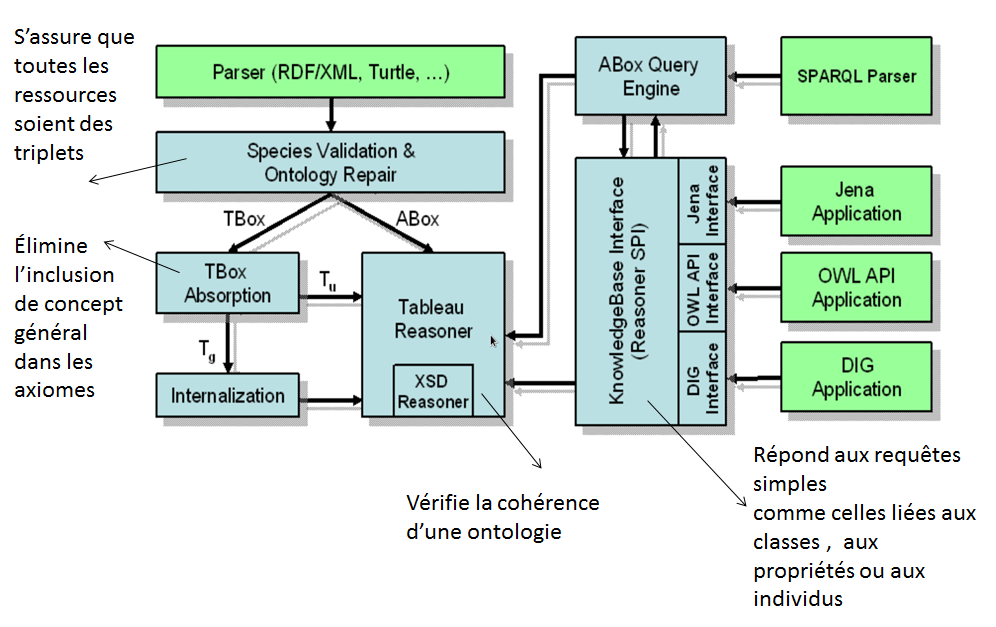
\includegraphics[scale=0.7]{reasoner.png}
\captionof{figure}{Principaux composants du \textit{reasoner} Pellet}
\end{center}

\paragraph{Inférences produites}
En vérifiant la cohérence d'une ontologie, les \textit{reasoner} peuvent déduire de nouvelles relations entre les concepts. Ces déductions ont correspondent à l'application de la logique qui vérifie la cohérence.

\paragraph{Évaluation de l'option}
Après avoir étudié différents \textit{reasoner open source} comme FaCT++, Pellet, Jena, cette solution a été écartée car, de mon point de vue, elle ne correspondait pas à l'exigence des demandes. En effet, avec les \textit{reasoners} actuels qui agissent comme des boites noires, l'utilisateur n'a pas le contrôle sur les inférences produites. Les \textit{reasoner} ont pour but premier de vérifier la cohérence et non d'inférer sur données. Par ailleurs, une autre demande du cahier des charges que l'on m'a confié, était la préférence de Logilab pour le langage Python. Or, pour le moment, aucun \textit{reasoner} n'est codé en Python.


    

\subsection{Les systèmes experts}
\paragraph{}
Après avoir écarté l'option des \textit{reasoner}, j'ai proposé les systèmes experts. Un système expert reproduit les mécanismes cognitifs d'un expert dans un domaine particulier. Un système expert est composé de trois parties. (Cf le schéma ci-dessous)
\begin{multicols}{2}
\begin{center}
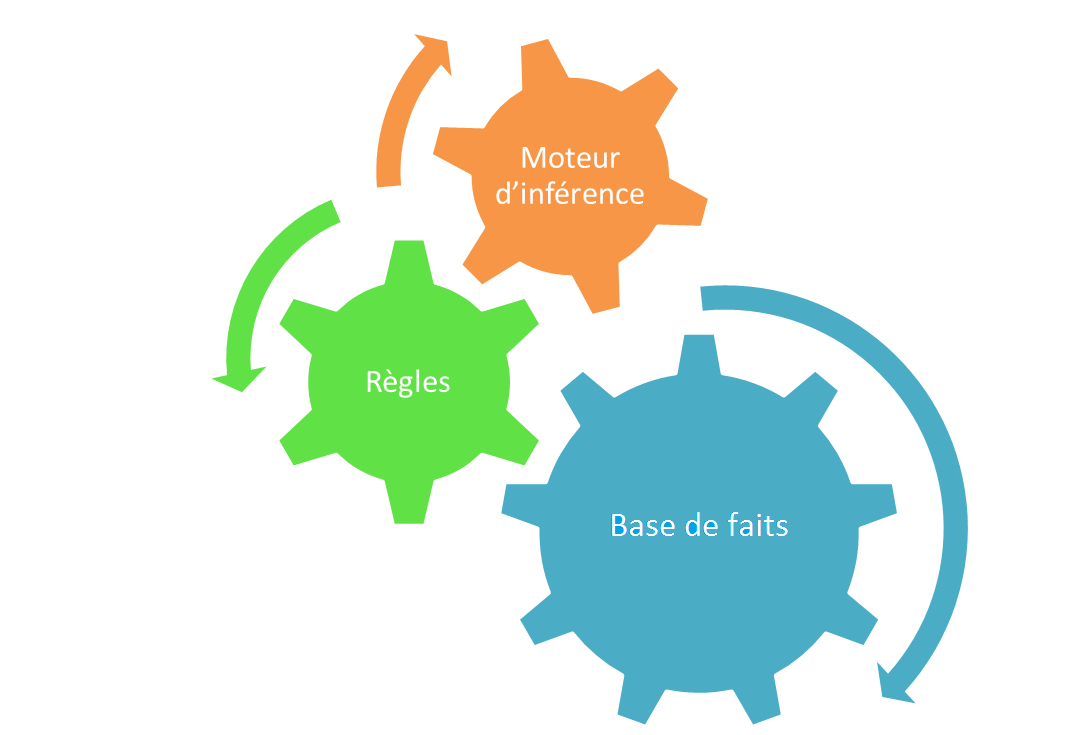
\includegraphics[scale=0.3]{se.png}
\end{center}

\paragraph{La base de faits}
La base de faits regroupe un ensemble de connaissances considérées comme vraies appelés "fait". Il existe deux types de faits : les faits spécifiques et les faits universels. Les faits spécifiques correspondent à des données propres au problème en cours. Les faits universels sont considérés comme toujours vrai indépendamment du problème.


\paragraph{Les règles}
Il existe deux types de règles : 
\begin{itemize}
    \item Les règles en \textbf{chaînage avant} : méthode de déduction qui part des prémisses pour déduire de nouvelles conclusions
    \item Les règles en \textbf{chaînage arrière} : méthode de déduction qui part des conclusions et tente de remonter aux axiomes.
\end{itemize}
\end{multicols}

\paragraph{Le moteur d'inférence}
Le moteur d'inférences peut déduire de nouveaux faits et répondre à une question en ajoutant de nouveaux faits déduits dans la base de fait (méthode par saturation) ou non.

\subsubsection{Exemple d'un système expert}

\begin{tabular}{|l|}
\hline
\\
\textbf{Base de faits}\\
Pierre est le père de Jean\\
Jean est le frère de Simon\\
Nathalie est la mère de Simon\\
\\
\textbf{Base de règles}\\
Si x est frère de y alors la mère de x est aussi la mère de y\\
Si x est frère de y alors le père de x est aussi le père de y\\
\\
\textbf{Le moteur d'inférences déduirait les faits suivants}\\
Nathalie est la mère de Jean\\
Pierre est le père de Simon\\
\hline
\end{tabular}

\paragraph{}
Cette proposition a été étudiée par le département pour sa capacité à être appliquée à tous les cas particuliers, sa flexibilité, le contrôle des déductions et son implémentation possible en Python. Néanmoins, construire des règles pertinentes nécessite une expertis approndie. Or dans le cas d'une application CubicWeb, le modèle métier est définit par le client. Or ce dernier ne possède pas systématiquement les compétences pour construire des règles.


\subsection{Les bases de données déductives}
\paragraph{}
Une base données déductive est une base de données capable d'effectuer des déductions à la manière d'un système expert, c'est-à-dire en utilisant des faits et des règles stockés dans la base de données déductive. Elle combine le paradigme de la programmation logique et les bases de données relationnelles. Aujourd'hui, les nouvelles applications des bases de données déductives sont l'intégration de données, l'extraction d'information, les réseaux sociaux, l'analyse de programmes, la sécurité et le \textit{cloud computing}\footnotemark[1]. Dans le cas du développement des applications \textit{CubicWeb}, cette solution est extrêmement pertinente car elle offre les mêmes avantages que les systèmes experts, avec une possibilité d'ajout de fonctions logiques. Deplus, les bases de données déductives ont été pensées pour travailler avec des bases de données. Dans l'optique de la spécialisation en Python de Logilab, l'étude du module Python PyDatalog a été engagée.

\footnotetext[1]{\textit{Cloud computing} : technologie qui permet de mettre sur des serveurs localisés à distance des données de stockage ou des logiciels.}


\chapter{Création du cube système expert}
\section{Objectifs et cas d'utilisation}
\begin{multicols}{2}
\begin{center}
\flushright
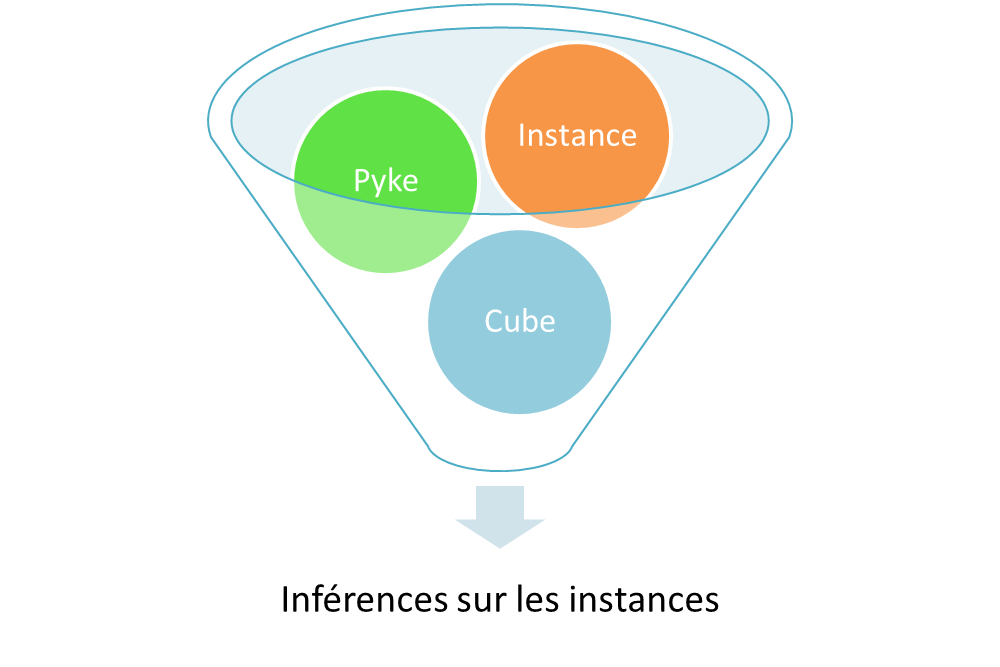
\includegraphics[scale=0.5]{pyke.png} 
\end{center}
\subsection{Objectifs}
\paragraph{}
Le cube \textit{Expert System} est un cube métier qui a pour rôle de fournir à un autre cube applicatif la possibilité d'y introduire des systèmes experts. Ce mécanisme permettra d'apporter des raisonnements inductifs simples. Le cube \textit{Expert System} utilise le module Python PyKE. Dans un premier temps, comprendre le fonctionnement de Pyke a été déterminant pour réaliser le cube \textit{Expert System}. Pyke fournit un mécanisme d'inférences de connaissances, écrit en Python, basé sur le modèle du système expert. Il est inspiré de Prolog et apporte des possibilités de programmation logique. Néanmoins, contrairement à Prolog, Pyke s'intègre parfaitement à Python. Grâce à un ensemble de règles, le moteur d'inférences PyKE infère sur la base de faits fournie par la base de données du cube applicatif \textit{CubicWeb} via l'instance du cube applicatif. 
\end{multicols}

\subsection{Cas d'utilisation}
\paragraph{}
Dans un forum, un commentaire peut commenter une discussion ou un autre commentaire. Or dans une chaîne de commentaire, le commentaire n'est pas rattaché au sujet de la discussion mais à un autre commentaire, lui même pouvant petre rattaché à un commentaire et ainsi de suite jusqu'au commentaire initial qui est rattaché au sujet de la discussion (Cf schema ci-après). Le système expert permet de déduire à quel sujet n'importe quel commentaire est rattaché.

\begin{center}
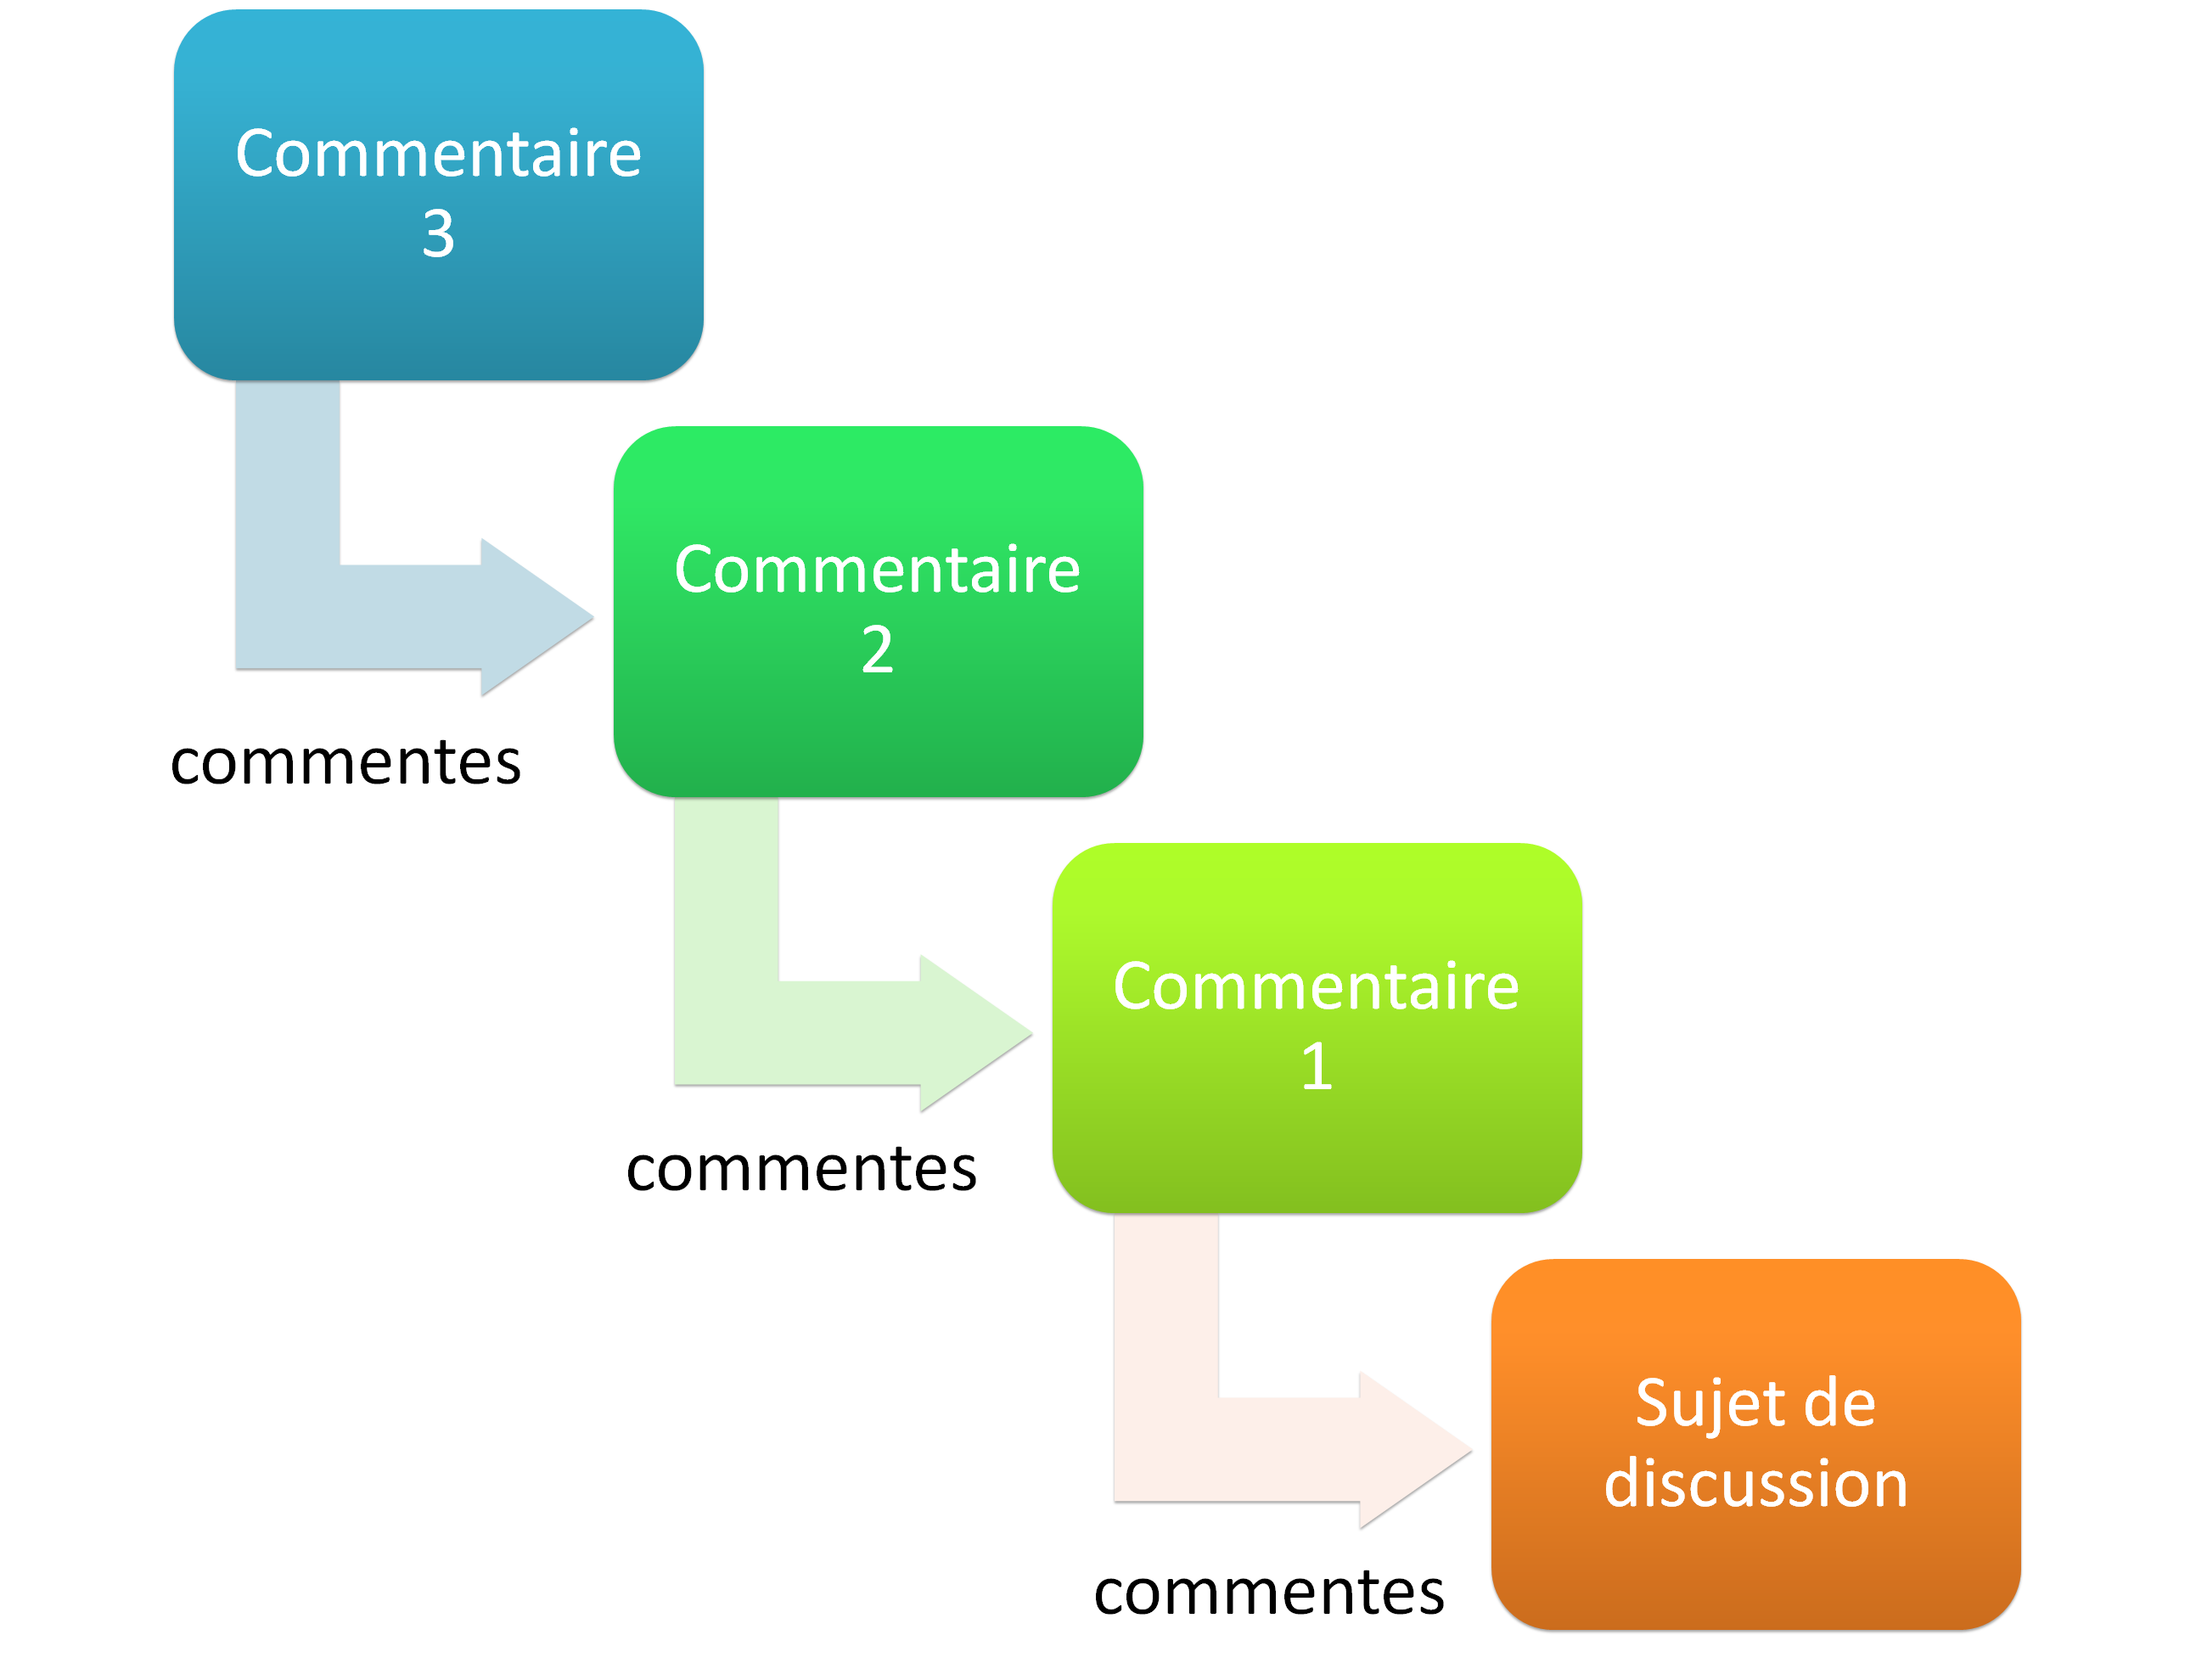
\includegraphics[scale=0.1]{chain.png}
\captionof{figure}{Chaîne de commentaires}
\end{center}

\section{Base de faits}

\subsection{Les faits issus du Cube Forum}
\paragraph{}
Les faits sont modélisés par le schéma du cube \verb+Forum+ ci-dessous : 

\renewcommand{\lstlistingname}{Code}
\begin{lstlisting}[caption= Schéma du cube Forum]
class ForumThread(EntityType):
    title = String(required=True, fulltextindexed=True, maxsize=256)
    content = RichString(required=True, fulltextindexed=True)
    in_forum = SubjectRelation('Forum', cardinality='1*', inlined=True,
                               composite='object')

class Comment(EntityType):
    """a comment is a reply about another entity"""
    content = RichString(required=True, fulltextindexed=True)
    comments = SubjectRelation('Comment', cardinality='1*',
                                          composite='object')
    in_thread = SubjectRelation('Comment', cardinality='?*',
                                           composite='object')

class comments(RelationDefinition):
    subject = 'Comment'
    object = ('ForumThread', 'Comment')
    cardinality = '1*'
\end{lstlisting}

Les faits ont alors la forme suivantes:
\begin{itemize}
\item L'entité X commentes l'entité Y
\item X est un commentaire
\item X est un sujet de discussion
\end{itemize}

\paragraph{Fonctionnement de Pyke}
Le fonctionnement de Pyke ne permet pas à un fait d'être dupliqué. Une tentative d'ajout d'un fait déjà existant sera ignoré. Un fait est considéré comme immuable : il ne peut pas être modifiés ou rétractés. Chaque fait à un nom et un tuple d'arguments. Ses arguments sont des données Python. Contrairement aux faits universels qui ne sont jamais supprimés, les faits spécifiques seront supprimés lors de la réinitialisation du moteur de Pyke. En effet, Pyke peut réinitialiser son moteur d'inférences et ainsi le dernier ensemble de faits est supprimé.


\subsection{Constitution de la base de faits}
\paragraph{}
On ajoute un fait spécifique ou un fait universel de la manière suivante :
\begin{itemize}
    \item \verb+some_engine.add_case_specific_fact(kb_name, fact_name, arguments)+
    \item \verb+some_engine.assert_(kb_name, fact_name, arguments)+    
\end{itemize}
\paragraph{}
La base de faits est construite en interrogeant la base de données existante par requêtes RQL.
\renewcommand{\lstlistingname}{Code}
\begin{lstlisting}[caption= Création de la base de faits]
def push(engine, _rql,base_name, relation, entity):
    for r in _rql:
        if len(r) == 2:
           engine.assert_(base_name, relation, (r[0], r[1]))
        else:
           engine.assert_(base_name, entity, (r[0], 0))        
\end{lstlisting}
\paragraph{}
Les faits issus de la requête RQL sont de deux types : relation (eg : X comment Y ) ou entité (eg : X is Forum). Si la requête porte sur une relation alors le résultat renvoie les identifiants (\verb+eid+) des deux membres de la relation et la longueur sera de 2. Dans le cas où la requête porte sur une entité, le résultat renvoie l'identifiant (\verb+eid+) de l'élément et la longueur de r est 1. Suivant ce résultat, on ajoute les faits différemment dans la base.

\subsection{Mise à jour des faits}
Afin de garder une base de faits cohérentes, sa mise à jour est indispensable. En effet, l'ajout d'un commentaire ou d'un sujet de discussion (ou leurs suppressions) va modifier la base de faits. Ainsi, le \textit{hook} du cube applicatif appelle le fichier \verb+sePyke.py+, chargé du lancement du système expert lors de l'ajout ou de la suppression d'un fait de la base. Cela permet de mettre à jour la base de faits à la création ou à la suppression d'un fait. En voici un exemple : 
\begin{lstlisting}[caption= Hook du cube forum gérant l'activation du système expert]
class ExpertSystemAfterAddComment(hook.Hook):
    """automatically activate the expert system after adding a comment"""
    __regid__ = 'forum.expert_system_after_add_comment'
    events = ('after_add_entity',)
    __select__ = hook.Hook.__select__ & is_instance('Comment',)

    def __call__(self):
        driver_forum(self._cw)
\end{lstlisting}

\paragraph{}
Cette classe est utilisée après l'ajout de l'entité \verb+Comment+. Elle appelle alors le pilote situé dans le fichier \verb+sePyKE.py+ et permet le lancement du système expert à chaque ajout d'entité.
\section{Base de règles}

\subsection{Les règles}
\paragraph{}
Les règles sont écrites dans un fichier.krb. Une règle est composée de prémisses et de conclusions. Pyke permet d'établir plusieurs conclusions. Le fichier .krb peut contenir des règles de type chaînage-avant et des règles de type chaînage-arrière. Pyke les différenciera car elles n'ont pas la même syntaxe. Les règles de type chaînage-avant possèdent les mots clefs \verb+assert+ et \verb+foreach+ qui correspondent au raisonnement "Si/Alors". Les règles de type chaînage-arrière sont écrites à partir des mots clef \verb+use+ et \verb+when+ qui correspond au raisonnement "utilise ce fait si".


Pour déterminer à quel sujet de discussion est rattaché un commentaire, deux règles sont nécessaires :
\begin{itemize}
\item une première règle qui définit la transitivité d'un commentaire : si X commente Y, Y comment Z alors X commente Z. 
\item une deuxième règle qui indique à quel sujet de discussion appartient un commentaire : Si Y est un sujet de discussion et X commente Y alors X appartient au sujet de discussion Y.
\end{itemize}


\subsection{Constitution de la base de règles}
Dans l'optique de conserver un maximum de code Python, la fonction \verb+driverBuilder()+ génère le fichier .krb, propre à Pyke, où sont stockés les règles. On obtient la base de règle suivante :

\begin{lstlisting}[caption= Base de règle du cube Forum]
comments_chains
	foreach
		comment_base.comments($Y, $Z)
		comment_base.comments($X, $Y)
		check $Y != $Z
		check $X != $Y
	assert
		comment_base.comments($X, $Z)

in_thread
	foreach
		comment_base.ForumThread($Y, 0)
		comment_base.comments($X, $Y)
		check $X != $Y
	assert
		comment_base.in_thread($X, $Y)
\end{lstlisting}

\paragraph{}
La première règle \verb+comments_chains()+ définit la transitivité d'un commentaire : si X commente Y, Y comment Z alors X commente Z. La règle \verb+in_thread()+ indique à quel sujet de discussion appartient un commentaire : Si Y est un sujet de discussion et X commente Y alors X appartient au sujet de discussion Y.




\section{Moteur d'inférences}

\paragraph{}
La mise en place du système expert est effectuée dans un fichier Python (\verb+sePyke.py+). Elle suit les étapes suivantes : 
\begin{enumerate}
    \item Constitution de la base de faits
    \item Constitution de la base de règles
    \item Activation du fichier contenant les règles
    \item Inférence de Pyke selon l'algorithme de chaînage avant par saturation.
\end{enumerate}
\paragraph{}
La constitution de la base de faits et de la base de règles ont été respectivement développées dans les paragraphes 8.2.2 et 8.3.2. Dans ce paragraphe, nous détaillerons l'activation des règles et le fonctionnement de Pyke qui lui permet d'inférer sur la base de faits.


\subsection{Activation des règles}
\paragraph{}
Un ensemble de règles est activé avec la commande \verb+some_engine.activate('monfichier')+. L'activation des règles n'est pas automatique. On active un fichier.krb à la fois. En effet, il peut en exister plusieurs. Créer plusieurs ensembles de règles permet de choisir entre les différentes bases de règles selon les situations spécifiques.

\subsection{Algorithme de chaînage-avant par saturation}
\paragraph{}
Les règles définies pour ce cas d'applications sont des règles de type chaînage-avant : \textit{"if A B C then D E"}. Afin de pouvoir déduire à quel sujet de discussion est rattaché un commentaire, Pyke suit l'algorithme de chaînage-avant par saturation, expliqué ci-après. Si les règles avaient été de type-chaînage arrière, Pyke aurait suivi un algorithme de chaînage-arrière. Ce dernier se trouve en Annexe A.1.

\begin{multicols}{2}

\paragraph{}
Une correspondance est recherchée entre la prémisse et les faits connus. Cette correspondance est déterminée par un mécanisme de \textit{Pattern variables}, décrit dans le paragraphe suivant. Pyke essaye toutes les combinaisons possibles à travers le procédé de chaînage-arrière. Potentiellement, une règle peut réussir plusieurs fois. Si Pyke réussit à trouver une correspondance pour une prémisse, il va tenter de traiter la prémisse suivante dans la liste. Si la dernière prémisse a une correspondance alors la règle est appliquée. Si Pyke échoue sur une prémisse, il remonte à la prémisse précédente dans la liste et trouve une autre solution. S'il remonte jusqu'à la première prémisse et échoue alors la règle échoue.

\begin{center}
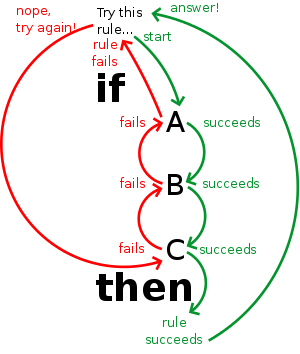
\includegraphics[scale=0.7]{if-then.png}
\captionof{figure}{Algorithme de chaînage-avant}
\end{center}

\end{multicols}
\paragraph{}
L'algorithme de Pyke fonctionne par saturation. Un moteur en chaînage-avant fonctionnant par saturation boucle sur la base de règles tant que de nouveaux faits peuvent être rajoutés dans la base de faits. L'algorithme prend en entrée la liste des faits et la liste des règles et ajoute les faits intermédiaires déduits dans la base de faits.

\subsection{Pattern Matching}
\paragraph{}
Le \textit{Pattern Matching} est un mécanisme qui vérifie si les données peuvent correspondre. Il est indispensable pour généraliser les faits. Il existe deux mécanismes de vérification : le \textit{Literal Patterns} et le \textit{Pattern variables}. Les \textit{Literal patterns} sont des valeurs qui ne correspondent qu'à elles-mêmes. Par exemple, pour vérifier qu'un fait est vrai, tous les arguments du fait seront considérés comme des \textit{Literal Pattern}. Pyke regardera alors si les arguments correspondent parfaitement aux arguments d'un fait contenu dans sa base. Les \textit{Pattern variables} sont des valeurs de données qui peuvent correspondre avec n'importe quelle donnée ou variable. Contrairement aux \textit{Literal Pattern}, les \textit{Pattern variables} permettent de répondre à une requête ouverte et non à une requête booléenne. Par exemple, si on souhaite savoir \textit{"Comment s'appelle le fils de Florence et Philippe ?"}, on écrira le fait ainsi : family.son\_of(\$son, Florence, Philippe). Les variables sont obligatoirement précédées du symbole \$ pour que Pyke puisse les identifier comme \textit{Pattern variables} et puisse effectuer le \textit{Pattern Matching}. Pour indiquer une variable dont on ne se préoccupe pas (variables anonymes), il faut précéder la variable du symbole "\$\_".














\section{Schéma du cube \textit{Expert System}}

\paragraph{}
Dans un premier temps, les notions de règles et de bases de faits étaient définies dans le schéma d'un cube comme suit pour permettre de créer des règles depuis l'interface de l'application (Cf figure 8.3):

\begin{lstlisting}[caption= Schéma d'un système expert]
class ExpertSystem(EntityType):
    name = String(maxsize=50, required=True, unique=True)
    description = RichString()

class Base(EntityType):
   name = String(maxsize=50, required=True, unique=True)
    description = RichString()
    in_expert_system = SubjectRelation('ExpertSystem', cardinality='1*',
                      		       composite='object')

class Rule(EntityType):
    name = String(maxsize=50, required=True, unique=True)
    description = RichString()
    in_base = SubjectRelation('Base', cardinality='1*',
                              composite='object')
    premisse = String(maxsize=1024, required=True)
    conclusion = String(maxsize=1024, required=True)
\end{lstlisting}

\begin{center}
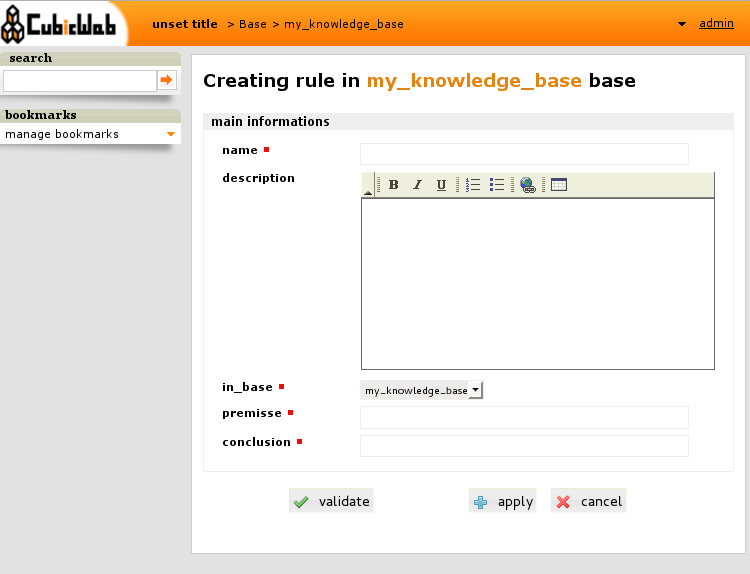
\includegraphics[scale=0.4]{se_rule_api.png}
\captionof{figure}{Interface pour la création d'une règle}
\end{center}

\paragraph{}
Dans une seconde version, les règles ne sont plus définies dans le schéma. Les règles nécessitent une expertise approfondie, et donc ne peuvent pas être créées à la volée. Elles ne seront donc pas définies via l'interface Web.








\section{Résultats obtenus}
\paragraph{}
Le cube métier \textit{Expert System} apporte bien la fonctionnalité d'inférences attendue. Ainsi l'écriture de la requête RQL \verb+Any X,Y WHERE Y in_thread X+ dans la barre de recherche affiche l'ensemble des commentaires liés au sujet A (Cf figure 8.4).

\begin{center}
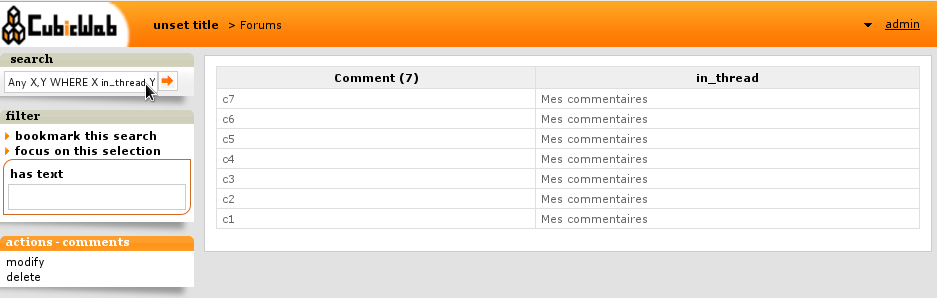
\includegraphics[scale=0.7]{in_thread.png}
\captionof{figure}{Résultat de la requête via l'interface de l'application}
\end{center}

\section{Apports personnels et pour Logilab}
\paragraph{}
La création de mon propre cube au sein de la plateforme CubicWeb m'a permis d'en cerner le fonctionnement. De plus, ce projet a nécessité la mise en œuvre de mon expertise et des connaissances acquises à l'UTC. Ce cube ouvre la voie à une approche logique et vers les systèmes experts.


\chapter{Réécriture de requêtes RQL}

\section{Les cas d'utilisations}
\paragraph{}
Le RQL propose un langage explicite de haut niveau permettant de faciliter leur utilisation. Cependant, selon le modèle de données, une requête peut être longue et complexe. Établir une correspondance entre un ensemble de relations et une relation simple, par exemple, permet d'alléger l'écriture. Les cas d'utilisations sont multiples : réécriture des relations complexes mais aussi réécriture d'attributs calculés, génération de paramètres génériques.

\subsection{La réécriture de relation}
Certaines relations sont complexes; le but de la réalisation est de les simplifier afin de faciliter l'expression syntaxique des requêtes. La requête ci-dessous permet, selon le modèle de données extrait du projet client pour la BnF, de sélectionner les illustrateurs A d'une œuvre B (ici appelé \verb+Manifestation+).

\renewcommand{\lstlistingname}{Requête}
\begin{lstlisting}[caption= sélection des illustrateurs d'une œeuvre donnée]
Any A,B WHERE C is Contribution, C contributor A, C manifestation B,
              C role R, R name "illustrator"
\end{lstlisting}
\paragraph{}
Le modèle de données établit qu'une personne contribue (\verb+contributor+) à une \verb+Manifestation+ selon un \verb+role+ (illusteur, auteur etc.). Avec la réécriture, cette requête peut être écrite comme suit. On constate que la simplification n'est pas dérisoire.
\renewcommand{\lstlistingname}{Requête avec réécriture}
\begin{lstlisting}[caption= requête RQL réécrite]
Any A,B WHERE A illustrator_of B
\end{lstlisting}

Cette réécriture s'intègre au modèle de données établi par CubicWeb. La définition de la règle de réécriture est intégrée au type de la relation \verb+illustrator_of+. Les types d'objets et de sujets sont inférés depuis la règle et ajouter à la définition de la relation. On appelle définition d'une relation le triplet <sujet> <relation> <objet>. Le type d'une relation sont les paramètres spécifiques à la relation seule.

\renewcommand{\lstlistingname}{Schéma}
\begin{lstlisting}[caption= Relation utilisant une règle de réécriture]
class illustrator_of(ComputedRelationType):
    rule  = ("C is Contribution, C contributor S, C manifestation O,
             C role R, R name 'illustrator'")
\end{lstlisting}

\subsection{Les attributs calculés}
Un attribut calculé est un attribut qui est déterminé par une requête RQL. Par exemple, la requête suivante sélectionne la somme des salaires versés aux salariés de chaque entreprise.

\renewcommand{\lstlistingname}{Requête}
\begin{lstlisting}[caption= Sélection de la somme des salaires]
Any SUM(SA) GROUPBY S WHERE P works_for S, P salary SA
\end{lstlisting}

Avec le principe de la réécriture, cette requête est réécrite comme suit:
\renewcommand{\lstlistingname}{Requête avec réécriture}
\begin{lstlisting}[caption= Sélectionne de la somme des salaires]
Any A WHERE S global_salary A
\end{lstlisting}

De même que pour la réécriture des relations, la réécriture des attributs calculés s'intègre au modèle de donnée CubicWeb:
\renewcommand{\lstlistingname}{Schéma}
\begin{lstlisting}[caption= Entité contenant un attribut calculé]
class Societe(EntityType):
    name = String()
    value = SubjectRelation('Mark')
    global_salary = Int(formula=("Any SUM(SA) GROUPBY S WHERE 
                                   P works S, P salary SA"))
\end{lstlisting}

\subsection{Le paramètre générique}
\paragraph{}
Il arrive que les instances d'une classe donnée n'aient pas de valeur à tous leurs attributs. Ue entité correspond à une tableau SQL où ses attributs sont des colonnes. Dans le cas où un attribut est peu rensigné, on obtient une colonne quasiment vide et ainsi une repésentation parcimonieuse. Définir un paramètre générique à la place d'utiliser un attribut classique évite d'obtenir un trop grand nombre de champs vides dans la table d'une entité. En effet, la colonne de l'attribut sera remplacé par des liens vers d'autres entités afin d'obtenir une meilleure optimisation. Ce paramètre générique possède un champ \verb+name+ et un champ \verb+value+. La relation \verb+has_parameter+ et la relation entre une ou plusieurs entités quelconques vers un paramètre générique.


\begin{lstlisting}[caption= Paramètre générique]
class CWParameter(EntityType):
    """Generic entity links an entity name to a value"""
    name = String()
    value = String()

class has_parameter(RelationDefinition):
    subject = '*'
    object = 'CWParameter'
    cardinality = '**'
\end{lstlisting}

\paragraph{Exemple}
Soit la classe \verb+Person+ avec l'attribute \verb+gender+. Or seulement un quart des instances de \verb+Person+ ont une valeur pour cet attribut. Dans ce cas, on utilise le paramètre générique. Cette solution est plus efficace dans ce contexte.


\begin{lstlisting}[caption= L'entité Person]
class Person(EntityType):
    name = String()
    gender = String(cw_parameter=True)
\end{lstlisting}

\paragraph{Paramètre générique et réécriture}
Dans le cadre du paramètre générique, les règles sont toutes identiques au modèle suivant: \verb+ S is A, S has_parameter C?, C name X, C value O+, où A est le type d'entité de S et X le nom du paramètre. La réécriture de la règle se fait donc automatiquement. La requête (1) pourra alors être remplacée par la requête (2)

\renewcommand{\lstlistingname}{Requête}
\begin{lstlisting}[caption= Paramètre générique et réécriture]
(1) : Any S WHERE S is Person, S has_parameter C?, C name 'gender',
      C value 'Male'
(2) : Any A WHERE A is Person, A gender "Male"
\end{lstlisting}

\paragraph{}
L'implémentation d'un tel paramètre est née de discussions sur des projets clients. Pour le moment, ce cas d'utilisation reste en suspens car il dépend largement des besoins client.

\section{Écriture de tests}
\paragraph{Test driven development}
Lors de ce stage, l'intérêt de la mise en place de tests automatiques m'a été fortement démontrée. En effet, cela permet de maintenir le code lors de son évolution. Lors d’un changement d’implémentation d’un module, si les tests unitaires passent, il y a de grandes chances pour que le reste de l’application continue à fonctionner. Pour la réécriture de requêtes RQL, mon développement a été piloté par les tests, suivant le principe du \textit{test driven development} (Cf figure XXX). Cette technique de développement consiste à prendre en compte un aspect particulier du problème, d'écrire un test couvrant cet aspect, d'écrire le code correspondant permettant de faire passer ce test, puis de faire passer le test et d'ajouter un nouveau test. Cette méthode offre un rythme soutenu au codage. Dans le cadre de la réécriture de requêtes RQL, plusieurs tests ont été implémentés en utilisant la bibliothèque de tests unitaires \verb+Unittest+. Cette bibliothèque fournit des fonctions qui testent le fonctionnement du code afin de vérifier si, par exemple, une fonction donnée lève une exception au moment voulu ou si deux objets sont égaux. 

\begin{center}
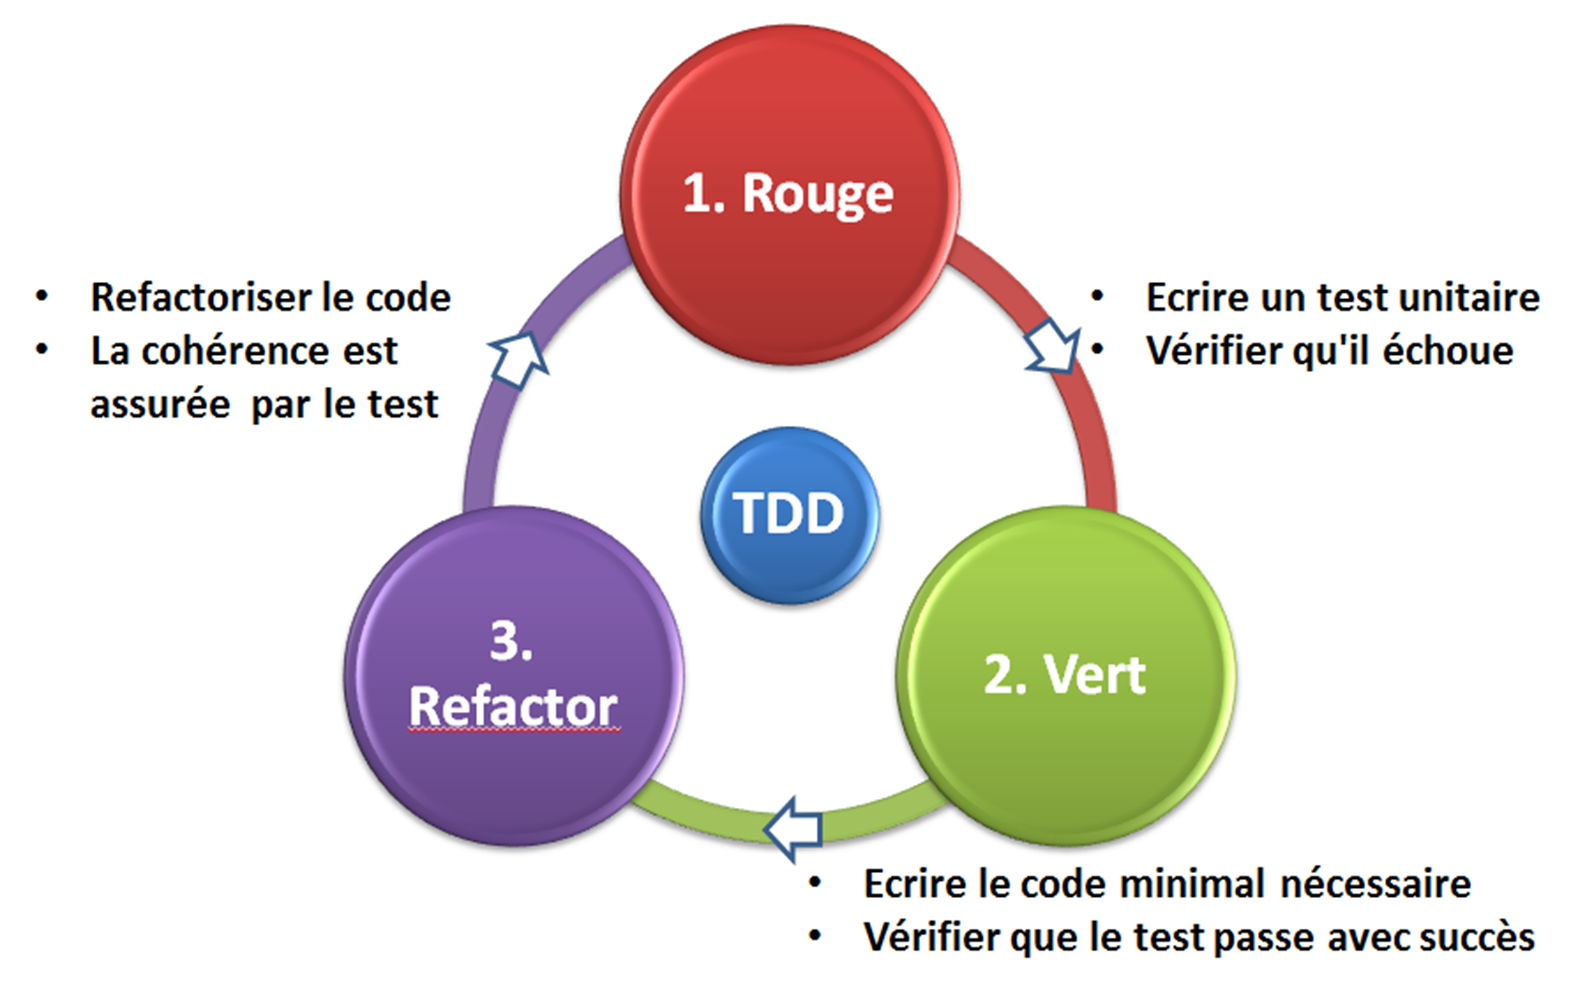
\includegraphics[scale=0.3]{tdd.png}
\captionof{figure}{Fonctionnement de la méthodologie\textit{Test driven development}}
\end{center}


\subsection{Réécriture de relation}
Dans le langage RQL, une relation peut être située à différents emplacements sur le graphe des requêtes. Les tests correspondent à la division du problème en sous-parties gérant les différents cas possibles:
\begin{enumerate}
\item Remplacer une relation située dans la partie conditionnelle \textsc{where}
\item Remplacer une relation située dans la sous-requête \textsc{with being} (exemple du test ci-dessous)
\item Remplacer une relation située dans une \textsc{union}
\item Remplacer une relation située dans une condition d'existence \textsc{exists}
\item Remplacer une relation située dans la partie conditionnelle \textsc{where} d'une requête de modification \textsc{set} ou de supression \textsc{delete} ou d'insertion \textsc{insert}
\item Permettre le remplacement récursif (exemple du test-ci-dessous)
\end{enumerate}
\renewcommand{\lstlistingname}{Test}

\begin{lstlisting}[caption= Relation située dans la sous-requête \textsc{with being}]
def test_rewrite_subquery(self):
    rule = {'illustrator_of': "C is Contribution, C contributor S, \
            C manifestation O, C role R, R name 'illustrator'"}
    tree = parse("Any A,B WHERE T relation C 
                  WITH A, B BEING(Any X, Y WHERE X illustrator_of Y)")
    r.rewrite(rule,tree)
    self.assertEqual(tree.as_string(),
                      "Any A,B WHERE T relation C 
                       WITH A,B BEING (Any X,Y WHERE D is Contribution, 
                       D contributor X, D manifestation Y, D role R,
                       R name 'illustrator')")
\end{lstlisting}


\begin{lstlisting}[caption= Remplacement récursif]
 def test_recursivity(self):
    rule = {'identify' : \verbatim{"S has C, C is Card, C value O"},
            'value' : "S is Number, S match O",
            'match' : "S match2 O"""}
    tree = parse("Any A,B WHERE A identify B")
    r.rewrite(rule,tree)
    self.assertEqual(tree.as_string(),"Any A,B WHERE A has C, C is Card, 
                     C is Number, C match2 B")
\end{lstlisting}

\paragraph{}
L'écriture des tests m'a permis de développer rapidement le programme Python de réécriture des requêtes, dont le code et l'algorithme sont en Annexe A.

\subsection{Réécriture d'attribut calculé}
De même, la mise en œuvre de la réécriture d'attributs calculés a été soumise à de nombreux tests. Les exemples ci-dessous gèrent respectivement l'utilisation d'un attribut calculé dans une fonction de comparaison et l'utilisation d'attribut calculé et de relation réécrite.

\renewcommand{\lstlistingname}{Test}
\begin{lstlisting}[caption= Attribut calculé et fonction de comparaison]
def test_computed_attribute(self):
        computed = {'salaire_total': 'Any SUM(SA) GROUPBY S WHERE
                                     P travaille S, P salaire SA'}
        tree = parse('Any S WHERE S salaire_total > 10000')
        r.rewrite(tree, None, computed)
        self.assertEqual(tree.as_string(), 'Any S GROUPBY S WHERE
                                            P travaille S, P salaire SA
                                            HAVING SUM(SA) > 10000')
\end{lstlisting}

\begin{lstlisting}[caption= Attribut calculé et réécriture de relation]
    def test_computed_attribute_and__rule(self):
        computed = {'salaire_total': 'Any SUM(SA) GROUPBY S WHERE
                                      P travaille S, P salaire SA'}
        rule = {'travaille' : 'S travaille_pour O'}
        tree = parse('Any A WHERE S salaire_total A')
        r.rewrite(tree, rule, computed)
        self.assertEqual(tree.as_string(), 'Any SUM(SA) GROUPBY S WHERE
                                            P travaille_pour S, P salaire SA')
\end{lstlisting}

\section{Intégration à la structure en place}

\subsection{Schéma Yams et CubicWeb}
\paragraph{Schéma Yams}
Pour construire et appliquer les règles aux requêtes RQL, le code écrit a dû être intégré à la structure de CubicWeb déjà en place. La règle pour être reconnue a dû être ajoutée au schéma Yams pour que les programmes reconnaissent les mots clés \verb+rule+, \verb+formula+, et \verb+cw_parameter+. Ainsi, j'ai ajouté un attribut \verb+rule+ au type d'une relation, et un attribut \verb+formula+ au schéma d'une entité. Les modifications apportées apparaissent en annexe XXX.

\paragraph{CubicWeb}
Le mécanisme de réécriture doit être appliqué avant les mécanismes de permissions et de sécurité de la requête, il a donc été appelé par le schéma CubicWeb dans un point de branchement suffisamment haut.

\subsection{Mises à jour des données}
\paragraph{Cohérence des données}
Dans une application, les données peuvent êre mises à jour très fréquemment. Dans le cas où une relation est réécrite, la requête RQL utilisant cette relation virtuelle déduira sa réponse et ne stockera pas la relation en base. La mise à jour des données n'aura donc pas de conséquences sur la cohérence des données liés à une relation réécrite. Au contraire, dans le cadre d'un attribut calculé, la valeur de l'attribut est calculé grâce à la formule et stocké en base. La modification d'une relation contenue dans la formule peut alors éventuellement changer la valeur de l'attribut calculé. J'ai donc implémenté un \textit{hook} qui met à jour la valeur d'un attribut calculé si une relation contenue dans sa formule est ajoutée ou modifiée.


\paragraph{Déclenchement de la mise à jour}
Le \textit{hook} se déclenche à l'ajout d'une relation (\verb+events=('after_add_relation')+) et si cette relation est contenue dans une formule d'un attribut calculé (\verb+__select__=match_computed_attribute()+). Cette seconde contrainte est construite avec la fonction \verb+match_computed_attribute()+ qui se trouve en annexe XXX.


\paragraph{Implémentation du hook}
Le \textit{hook} ci-dessous exécute la requête RQL de la formule de l'attribut calculé. La requête retourne alors la nouvelle valeur de l'attribut calculé ainsi que l'identifiant (\textit{eid}) de l'attribut calculé. Il lance alors la requête \verb+SET X attribut_calculé nouvelle_valeur WHERE X eid A+ où A est l'identifiant de l'attribut calculé. Le code complet de ce hook se trouve en annexe (XXX).

\paragraph{Migration des applications}
Les applications sont régulièrement mises à jours. Afin d'optimiser le coût en terme de performance de la migration d'une version à une autre, les données ne sont mises à jour que si nécessaire. Si d'une version à l'autre, la formule d'un attribut calculé change, il faut alors recalculer l'ensemble des attributs et ajouter les nouvelles valeurs au moyens d'une requête RQL de modification (\verb+SET+)

\subsection{Génération de tables SQL}
Dans le cadre de la réécriture, il était intéressant de ne pas générer la table d'une relation dont le seul but est de simplifier la réécriture. Après avoir compris le mécanisme, le programme de génération des tables SQL a été modifié en conséquence. Ces modifications se trouvent en annexe XXX.


\section{Communication autour du projet}
\paragraph{}
Le projet de réécriture de requêtes RQL modifie CubicWeb et \textit{Yams} et concerne l'ensemble des utilisateurs de ce framework. Il a donc nécessité d'établir un large plan de communication. Ainsi, j'ai rédigé des blogs en anglais sur l'intranet et sur \url{cubicweb.org} afin de communiquer essentiellement sur la finalité du projet et l'interface de programmation applicative envisagée. CubicWeb étant une plateforme \textit{open source}, j'ai également transmis ces informations à la liste de diffusions des utilisateurs de CubicWeb. Les utilisateurs de CubicWeb sont principalement les membres de Logilab mais aussi Softtek, une multinationale d'origine mexicaine. L'ensemble de la communication se fait donc en anglais. Ce devoir de communication m'a permis d'étendre mes compétences de rédaction sur un sujet technique, ce qui fut très enrichissant.




\section{Apports personnels et pour Logilab}
\paragraph{}
La réécriture de requêtes RQL permet à l'utilisateur de simplifier ses requêtes puisque le programme déduira, en fonction des règles, quelles relations appliquer. Cette mise en place d'une inférence d'un concept assez simple m'a permis : 
    \begin{itemize}
    \item de développer une fonctionnalité utile et appréciée pour toute l'entreprise
    \item de travailler sur le code de gestion de schéma (\textit{Yams}) de CubicWeb
    \item et de travailler selon une nouvelle méthode : \textit{test driven development}
    \end{itemize}
\paragraph{}
De plus, la possibilité de ne pas générer des tables SQL pour des relations "virtuelles" ouvre une voie pour une meilleure gestion des performances lors de l'exécution de requêtes.




\chapter{Réalisations secondaires}
\section{Vsprint}
\paragraph{Liste des sujets affectés}
 Voici la liste des sujets de Vsprint qui m'ont été attribués pendant les six mois de stage : 
\begin{itemize}
\item Correction d'anomalies de mise en forme sur le cube Bootstrap
\item Image search
\item Tracé en d3js du graphe des projets du tableau de bord
\end{itemize}

\paragraph{Imagesearch}
L'objectif de ce projet est de réaliser un navigateur qui parcourt une base d'images et restreint les images affichées par thème. En sélectionnant une image, on sélectionne un thème et on se rapproche ainsi peu à peu vers les images souhaitées. Ce projet est très intéressant car il propose une fonctionnalité de navigation alternative et dynamique.

\paragraph{Graphe des projets}
Ce projet consiste à mettre en place un graphe dynamique résumant l'avancée des différents projets client. Il m'a permis de découvrir d3js, une bibliothèque JavaScript dédiée à la manipulation de documents qui utilisent HTML, SVG\footnotemark[1] and CSS.
\paragraph{Bilan des Vsprint}
Les Vsprint m'ont permis de travailler en binôme sur des sujets divers et donc d'accroitre mes connaissances notamment sur Bootstrap, \textit{framework open source} de mise en forme de pages Web et les bibliothèques Javascript.

\footnotetext[1]{SVG (Scalable Vector Graphics) est un format d'image XML pour les graphiques à deux dimensions, qui supporte les interactivité et les animations.}


\section{Création d'un cube d'import CSV}
\subsection{Objectifs}
CSV est une repésentation des données tabulaires sous forme de valeurs séparées par des virgules ou par un quelconque séparateur comme un point-virgule. Il existait déjà un cube chargé de l'import CSV sous forme d'un tableau classique. L'objectif est de créer un nouveau cube métier et d'afficher les données tabulaires en utilisant  SlickGrid. SlickGrid est une bibliothèque Javascript permettant d'obtenir des tableaux plus élaborés. Le type de tableau attendu est un tableau capable de trier et filtrer les données, dont les dimensions sont fixes selon la page et disposant de barres de défilement.
\subsection{Implémentation}

\paragraph{Fonctionnalités implémentées}
\begin{itemize}
\item import du tableau
\item barre de défillement
\item formulaire d'options
\item filtres
\item possibilités de déplacement des colonnes par glissement
\end{itemize}

\begin{center}
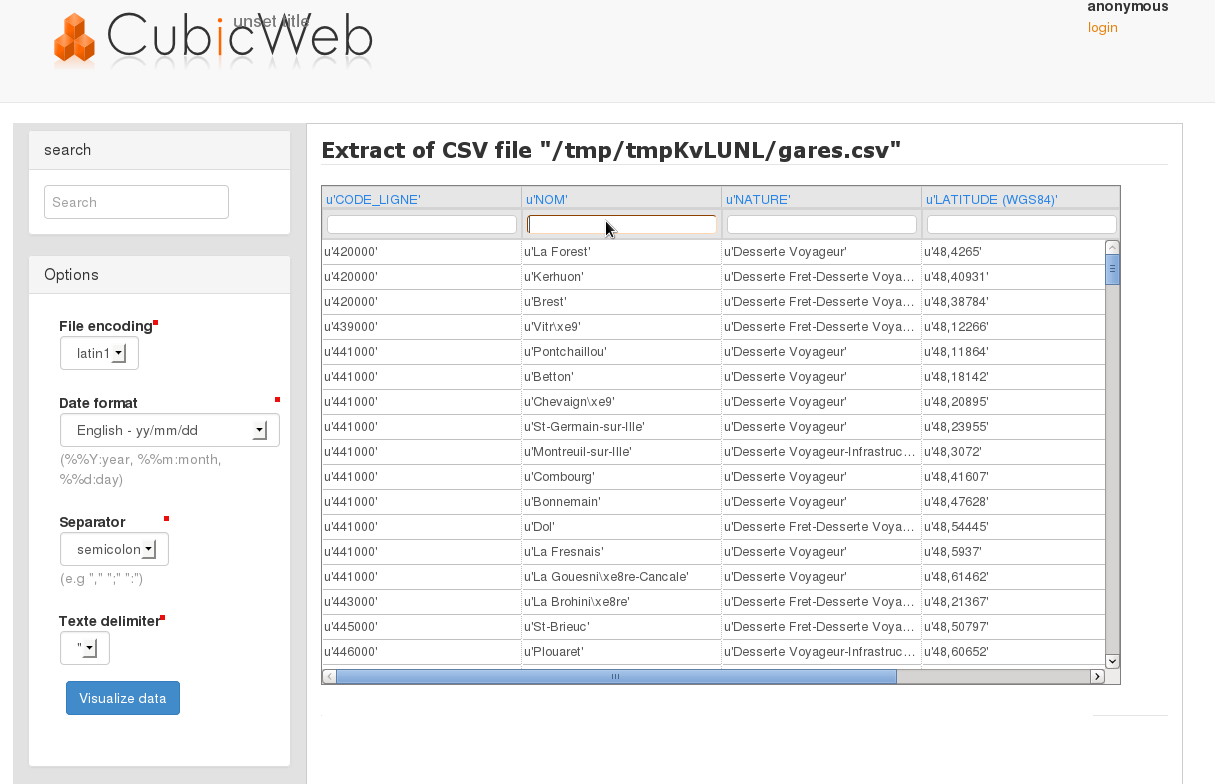
\includegraphics[scale=0.5]{slick.png}
\captionof{figure}{Interface du cube \textit{importcsv}}
\end{center}

\paragraph{Fonctionnement}
L'implémentation des barres de défillement, du formulaire d'options, des filtres et de la possibilités de déplacement des colonnes ont été réalisées à partir de bibliothèques javascripts. Pour obtenir un fichier CSV sous forme de tableau présentable, il a fallu décoder le fichier afin de déterminer le type de séparateur (espace, virgule, point-virgule etc.). Puis, les données sont stockés dans une matrice.

\begin{lstlisting}[caption= code à insérer]
\end{lstlisting}


\paragraph{Apports personnels et pour Logilab}
Ce projet m'a permis d'améliorer mes connaissances et ma pratique du javascript\footnotemark[1]. Il fut également enrichissant par ma découverte de la bibliothèque SlickGrid et m'incite à découvrir les nouveautés dans le milieu de l'\textit{open source}. Pour Logilab, ce cube métier sera très utile. En effet, de nombreux projets client requièrent un import CSV, une mise une page compacte des tableaux, et des tableaux aux fonctionnalités évoluées. Une mise en forme compacte permet d'afficher le tableau sans faire défiler l'ensemble de l'écran, bien que ce dernier ait trois mille lignes.


\footnotetext[1]{javascript : langage de programmation de scripts utilisé dans les pages Web interactives}

\chapter{Conclusion}
\paragraph{}
Ce stage au sein de Logilab a été une expérience très profitable. La richesse et l'originalité du sujet m'ont séduites. Mettre en place des inférences au sein d'un logiciel comme CubicWeb a été un véritable défi. 

\paragraph{}
Ces vingt-quatre semaines ont été extrêment instructives au niveau de la méthodologie et des outils utilisés. J'ai pu appliquer la méthodologie agile, méthodologie très répandue dans les projets informatiques, et constater son efficacité pour s'assurer de la satisfaction du client. J'ai également pu en cerner les limites : sa réussite dépend de la disponibilité du client. De même, mon travail a été soumis à la méthodologie du \textit{test driven development} où l'implémentation est guidée par des tests unitaires. Cette méthode m'a semblé très efficace pour générer du code rapidement et conserver une vérification des résultats en cas de changement d'implémentation. De plus, l'utilisation d'un gestionnaire de versions décentralisé comme Mercurial fut une remarquable découverte et je compte l'appliquer à mes projets futurs.

\paragraph{}
Le sujet de ce stage correspond à un travail de recherche pour le développement interne et consistait à apporter une plus-value à l'entreprise. Ma mission, pour un client interne, à savoir le comité de pilotage de CubicWeb, a été soumis aux mêmes problématiques que pour un projet client classique. En effet, il est fréquent que le client ne sache pas toujours ce dont il a réellement besoin. Confrontée à ce problème, j'ai appliqué les méthodes agiles et le projet a été réorienté sur les besoins réels. De même, la communication est au cœur de la relation client, afin d'expliquer les apports fonctionnels des changements proposés et éviter les incompréhensions. Ce devoir de communication et d'agilité, parti intégrante du métier d'ingénieur, fut très enrichissant. De plus, ayant très peu travaillé en équipe, ce contexte m'a permis de prendre de l'indépendance, de l'autonomie, et de réfléchir sur les besoins de l'entreprise.

\paragraph{}
Les difficultés rencontrées résident dans la mise en place du projet puisque le sujet de stage reste prospectif. Toutefois les spécifications se sont précisées au fil des études et démonstrations que je leur ai apporté. CubicWeb étant utilisé par l'ensemble des membres de Logilab, de nombreux avis, parfois divergents, ont réorienté le projet. Je pense néanmoins avoir réussi à faire avancer le projet et CubicWeb.

\paragraph{}
Travailler sur CubicWeb m'a permis de me plonger dans le domaine de la gestion de connaissances. Cela a confirmé mon désir de me spécialiser dans le domaine de l'Ingénieurie de Connaissances et Systèmes d'Information.


\appendix


\chapter{Algorithmes}
\section{Algorithme de chaînage-arrière}

\paragraph{Struture et fonctionnement}
Les règles en chaînage-arrière sont traitées quand le programme demande à Pyke de prouver un but précis. Pour établir cette preuve, Pyke utilisera uniquement les règles déjà activées. Pour faire du chaînage-arrière, Pyke essaye récursivement de prouver tous les sous-buts. Quand tous les sous-buts sont prouvés, la règle aboutit et le but est prouvé.

\paragraph{Algorithme de chaînage-arrière}
    L'algorithme de chaînage-arrière procède comme suit : 
\begin{itemize}
    \item Si la règle ne conduit pas à une correspondance avec la base de faits alors elle échoue et elle remonte au nœud précédent dans le graphe.
    \item Si la règle conduit à une correspondance avec la base de faits alors elle réussit et crée une nouveau nœud dans le graphe des solutions.
\end{itemize}

\paragraph{}
Cet algorithme inclut toute la chaîne d'inférence depuis le tout début pour prouver le but final. L'avantage d'un tel algorithme est sa capacité à retourner sur n'importe quel nœud du graphe pour trouver une solution alternative. Les règles sont appliquées dans l'ordre, il est donc préférable de mettre les règles qui ont le plus de chances de s'appliquer en premier.

\paragraph{}
L'algorithme de chaînage-arrière est en profondeur d'abord. En effet, il s'agit d'un parcours où l'on explore le graphe jusqu'à ce que l'on ne puisse plus appliquer une règle. Ce cas survient lorsque l'on a parcouru tout le graphe ou lorsque l'on est arrivé sur un nœud qui n'a pas de successeurs. Dans ce cas, l'algorithme retourne au nœud précédent et cherche un nœud qui n'a pas encore été visité. L'algorithme complet se trouve ci-dessous :
\begin{tabbing}
\textit{Fonction chaînage arriere}\\
Paramètres : in BR, in BF, in listeButs.\\
\hspace{0.5cm} \= \hspace{0.5cm} \= \hspace{0.5cm} \= \hspace{0.5cm} \= \hspace{0.5cm} \= \kill
\> \textbf{if} est vide(listeButs) \textbf{then}\\
\> \> res $\leftarrow$ SUCCES\\
\> \textbf{else}\\
\> \> \textbf{if} demBut(premier(listeButs)) \textbf{then}\\
\> \> \> res $\leftarrow$ chaînageArriere(suite(listeButs))\\
\> \> \textbf{else}\\
\> \> \> res $\leftarrow$ ECHEC\\
\> \> \textbf{end if}\\
\> \textbf{end if}\\
retourner res\\
\end{tabbing}

\begin{tabbing}
\textit{Fonction demBut}\\
Paramètres : in BR, in BF, in but.\\
\textbf{if but $\in$ BF then}\\
\hspace{0.5cm} \= \hspace{0.5cm} \= \hspace{0.5cm} \= \hspace{0.5cm} \= \hspace{0.5cm} \= \kill
\> res $\leftarrow$ SUCCES\\
\textbf{else}\\
\> regles $\leftarrow$ BR; res $\leftarrow$ ECHEC\\
\> \textbf{while} regles = $\varnothing$ et res = SUCCES do\\
\> \> r $\leftarrow$ choix(regles); regles $\leftarrow$ regles - {r}\\
\> \> \textbf{if conclusion(r) = fait then}\\
\> \> \> res $\leftarrow$ chaînageArrière(BR, BF, premisse(r))\\
\> \> \textbf{end if}\\
\> \textbf{end while}\\
\> retourner res\\
\textbf{end if}\\
\end{tabbing}
\paragraph{}

\chapter{Code}
\section{Hook de mise à jour des données d'un attribut calculé}
\renewcommand{\lstlistingname}{Hook}
\begin{lstlisting}[caption= Mise à jour des données d'un attribut calculé]
class ComputedAttributeHook(SyncSchemaHook):
	"""After adding relations which are in a computed attribute rule,
	the computed attribute is filled thanks to the rule."""
	__regid__ = 'schema.computed_attribute_after_add_entity'
	__select__ = SyncSchemaHook.__select__ & match_computed_attribute()
	events = ('after_add_relation',)

	def __call__(self):
		operation = SyncSchemaComputedAttributeOperation.get_instance(self._cw)
		operation.add_data((self.eidfrom, self.rtype, self.eidto))
		operation.postcommit_event()

class SyncSchemaComputedAttributeOperation(hook.DataOperationMixIn, hook.Operation):
	def postcommit_event(self):
		session = self.session
		schema = session.repo.vreg.schema
		for self.eidfrom, self.rtype, self.eidto in self.get_data():
			for entity in schema.entities():
				for attr in entity.attribute_definitions():
					formula = attr[0].formula
					if formula and self.rtype in formula:
						rql = hook_rewrite_computed(formula, self.eidfrom, 
									self.rtype, self.eidto, schema.get_rules())
						rset = session.execute(rql)
						if rset:
							for r, eclass in rset.rows:
								if r:
									session.execute('SET X %(attr)s "%(r)s" 
									WHERE X eid %(eclass)s'
									% {'attr': attr[0], 'r': r, 'eclass': eclass})
																	
		
\end{lstlisting}

\begin{lstlisting}[caption= Sélecteur]
class match_computed_attribute(EClassPredicate):
	"""Returns 1 if the relation is in the formula of a  computed attribute."""
	def __call__(self, cls, req, rset=None, **kwargs):
		rtype = kwargs.pop('rtype')
		schema = req.vreg.schema
		for entity in schema.entities():
			for attr in entity.attribute_definitions():
				if attr[0].formula:
					if rtype in attr[0].formula:
						return 1           
		return 0
\end{lstlisting}



\chapter{Glossaire}

\paragraph{Cloud computing}technologie qui permet de mettre sur des serveurs localisés à distance des données de stockage ou des logiciels.
\paragraph{CSS3}langage servant à décrire la présentation des documents HTML et XML.
\paragraph{CSV}format informatique ouvert représentant des données tabulaires sous forme de valeurs séparées par des virgules ou par un quelconque séparateur comme un point-virgule.
\paragraph{Cube}composant logiciel de base de CubicWeb, comportant trois parties principales : le modèle de données, la logique métier, l’interface utilisateur, ainsi que des dépendances vers d’autres cubes. 
\paragraph{CubicWeb}framework logiciel libre implémenté par l'entreprise Logilab.
\paragraph{Debian}système d'exploitation et une distribution de logiciels libres.
\paragraph{DOAP}vocabulaire RDF décrivant les projets logiciels.
\paragraph{FOAF}vocabulaire RDF permettant de décrire des personnes et les relations qu’elles entretiennent entre elles. C'est une application du Web sémantique.
\paragraph{Framework}ensemble de composants logiciels permettant de créer l'architecture d'un logiciel.
\paragraph{Hadoop}framework Java libre destiné à faciliter la création d'applications distribuées et échelonnables. Il permet aux applications de travailler avec des milliers de nœuds et des pétaoctets de données.
\paragraph{HTML5}cinquième version du format de données HTML conçu pour représenter les pages Web
\paragraph{Javascript}langage de programmation de scripts utilisé dans les pages Web interactives
\paragraph{Mercurial}logiciel de gestion de versions décentralisé qui administre les différentes versions d'un programme écrites par un ou plusieurs développeurs.
\paragraph{Moteur d'inférences}logiciel ou composant logicile correspondant à un algorithme de simulation des raisonnements déductifs.
\paragraph{Ontologie}Une ontologie est l'ensemble structuré des termes et concepts représentant le sens d'un champ d'informations. L'ontologie constitue en soi un modèle de données représentatif d'un ensemble de concepts dans un domaine, ainsi que des relations entre ces concepts.
\paragraph{Open data}données diffusées de manière structurée selon une méthodologie et une licence ouverte garantissant son libre accès et sa réutilisation par tous, sans restriction technique, juridique ou financière.
\paragraph{Open source}désigne un logiciel dont la license autorise la libre redistribution, l'accès au code source et la création des travaux dérivés.
\paragraph{Pattern variable}valeurs de données qui peuvent correspondre avec n'importe quelle donnée ou variable.
\paragraph{Pyke}Pyke est un moteur d'inférences de système expert, écrit en Python, qui introduit de la programmation logique inspirée de Prolog.
\paragraph{Python}langage de programmation orienté objet.
\paragraph{RDF}(Resource Description Framework) est un modèle de graphe destiné à décrire de façon formelle les ressources Web et leurs métadonnées, de façon à permettre le traitement automatique de ces descriptions.
\paragraph{Reasoner}programme capable d'inférer des conséquences logiques à partir de faits et d'axiomes et de vérifier qu'une ontologie est cohérente.
\paragraph{Responsive Design}notion de conception de sites Web qui permet à l'utilisateur de consulter le même site Web à travers une large gamme d'appareils (moniteurs d'ordinateur, smartphones, tablettes, TV, etc.) avec le même confort visuel.
\paragraph{RQL}(Relationship Query Language) langage informatique d'exploitation de bases de données, utilisé par \textit{CubicWeb}
\paragraph{SIOC}vocabulaire utilisant RDF permettant de décrire des objets couramment utilisés sur les sites communautaires et leurs relations.
\paragraph{Sparql}langage de requête et un protocole qui permet de rechercher, d'ajouter, de modifier ou de supprimer des données RDF disponibles à travers Internet.
\paragraph{Système experts}outil capable de reproduire les mécanismes cognitifs d'un expert, dans un domaine particulier.
\paragraph{W3C}(World Wide Web Consortium) est un organisme de normalisation à but non lucratif chargé de promouvoir la compatibilité des technologies.
\paragraph{Web sémantique}Le Web sémantique est un mouvement collaboratif mené par le World Wide Web Consortium (W3C) qui favorise des méthodes communes pour échanger des données. Le Web sémantique vise à aider l'émergence de nouvelles connaissances en s'appuyant sur les connaissances déjà présentes sur Internet.
\paragraph{Yams}signifie \textit{Yet Another Magic Schema}. C'est un module python qui définit le schéma générique des relations et des entités de manière simple et générique.
\paragraph{Vsprint}plage horaire hebdomadaire (les vendredi après-midi) où les membres du personnel travaillent en binôme sur un ensemble de tickets, généralement lié au développement d'outils internes.


\end{document}
